
\documentclass{article}
\usepackage{listings}
\usepackage[utf8]{inputenc}
\usepackage{graphicx}
\usepackage{subfiles}
\usepackage{wrapfig}
\usepackage{geometry}
\usepackage[italian]{babel}
\usepackage[export]{adjustbox}
\usepackage[font=scriptsize]{caption}
\usepackage{titlesec}
\usepackage{verbatim}
\setcounter{section}{-1}

\titlespacing*{\section}
{0pt}{3ex plus 1ex minus .2ex}{3ex plus .2ex}
\titlespacing*{\subsection}
{0pt}{3ex plus 1ex minus .2ex}{3ex plus .2ex}
\graphicspath{ {./images/} }
\geometry{a4paper, top=2cm, bottom=2cm, left=2cm, right=2cm, heightrounded, bindingoffset=5mm}
\hyphenation{duplicate ip address}


\title{\Huge LABORATORIO DI INTERNET 
    \\ Report individuale \\ 
    
    Analisi del comando \textit{nmap}}
\date{Maggio 2021}


\begin{document}
\lstloadlanguages{C}

\maketitle

\begin{center}
    
\includegraphics[scale=2.7]{logo_poli_nuovo.jpg}

    \vspace{10mm}

    Diego Zanfardino s256536 \\
    Gruppo 21

    \vspace{10mm}
    prof. Mellia Marco e Trevisan Martino 
\end{center}

\pagebreak
\section{Configurazione di rete}

\begin{figure}[h]
    \centering
    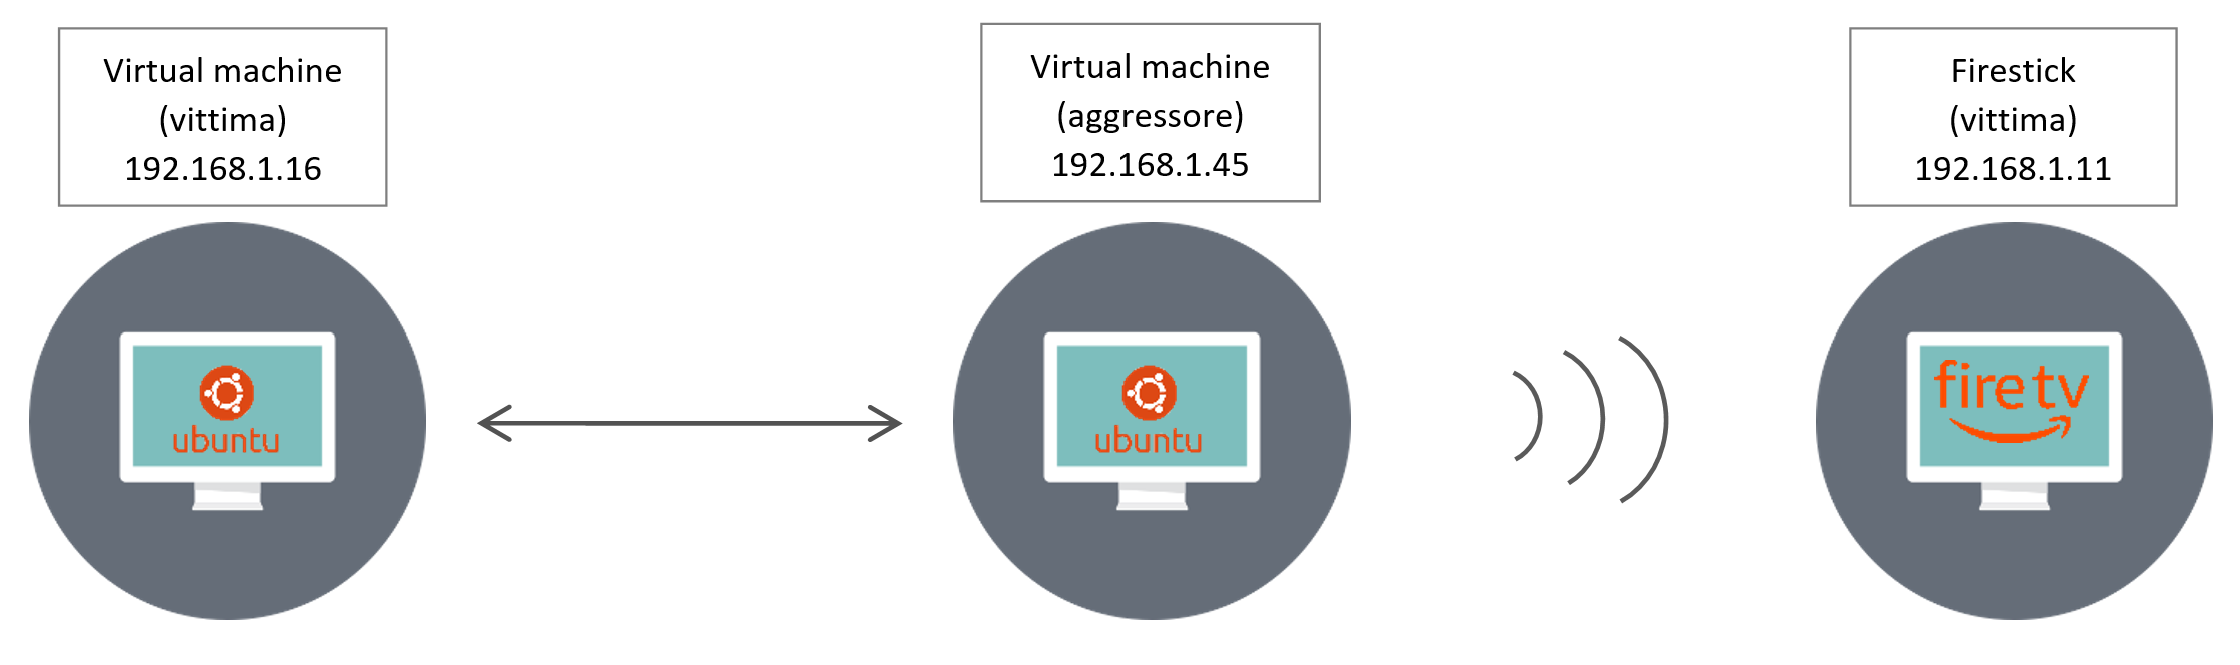
\includegraphics[scale = 0.5]{setup iniziale.png}
    \caption{Configurazione iniziale della rete}\label{Fig:data1}
\end{figure}
L'assegnazione degli indirizzi privati è affidata al DHCP del router 
a cui i dispositivi sono connessi. Tutti i dispositivi coinvolti appartengono
alla stessa sottorete. Le due virtual machine montano un sistema 
operativo linux-based (Ubuntu), mentre per conoscere il sistema operativo della 
Firestick è possibile sfruttare il comando \textit{"sudo nmap 192.168.1.11 -O"}
che fornisce come ipotesi un sistema operativo Android-based (4.X$\vert$5.X$\vert$6.X).


\section{Analisi delle prime 100 porte della virtual machine}
\subsection{Scan TCP}

\begin{wrapfigure}{l}{0.5\textwidth} %this figure will be at the right
  \centering
  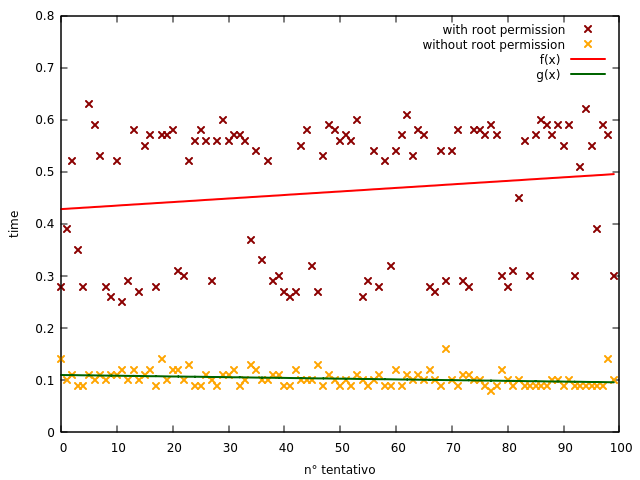
\includegraphics[width=0.5\textwidth]{sudo_vs_user_def.png}
  \caption{Sudo vs normal user}\label{Fig:sudovsuser}
\end{wrapfigure}

Il comando $$sudo\; nmap \;192.168.1.16\; -p \; 1-100$$ permette di eseguire uno scan delle prime 
100 porte TCP dell'indirizzo ip selezionato. Poichè il comando è eseguito come superuser
il comportamento di default è in modalita -sS (\textit{SYN Stealth}) che, sfruttando i privilegi
di root di poter creare pacchetti raw decidendone l'intestazione,
 manda pacchetti TCP SYN alla destinazione, in attesa di risposta con flag SYN-ACK (o RST-ACK). In caso di risposta 
affermativa, invece di chiudere la connessione con un pacchetto ACK, viene mandato un pacchetto
RST per chiudere bruscamente la connessione (da qui il nome di questo tipo di scan: \textit{half-open scanning}). 
Per essere più precisi è il \textit{kernel} della macchina che usa nmap a mandare il RST poichè non riconosce nel SYN-ACK mandato
dalla vittima nessun suo tentativo di aprire una connessione, essendo il pacchetto generato \textit{ad hoc} da nmap.
Questo tipo di comportamento è utile per destare meno sospetti nei confronti del firewall di rete aprendo diverse connessioni 
in un intervallo di tempo molto breve.
Avendo privilegi di root il comando \textit{nmap} può mandare ARP requests interfacciandosi 
direttamente con il livello rete, così da avere un riscontro certo se l'host sia attivo o meno, non potendo
il protocollo ARP rifiutare di rispondere ad una richiesta. Essendo eseguito come superuser si nota come la porta
sorgente sia la stessa per ogni pacchetto SYN mandato.\\
Nel caso in cui il comando venga eseguito senza permessi di root si fa uso della system call \textit{connect} che tenta di aprire la connessione
nel modo convenzionale, usando ogni volta una porta casuale tra quelle non assegnate dallo IANA. \\ Nel grafico in Figura 2 sono riportati i tempi 
di esecuzione per 100 comandi nmap verso lo stesso host, eseguiti sia come superuser che come utente normale. Sono inoltre rappresentate le due rette $f(x)$ e $g(x)$
che interpolano i punti ricavati, per cercare di ricavarne l'andamento macroscopico. Il tempo di esecuzione medio per la prima è di circa 0.428\textit{s}, mentre per
la modalità senza permessi di root è di circa 0.110\textit{s}

\begin{figure}%[!htb]
  \begin{minipage}{0.49\textwidth}
    \centering
    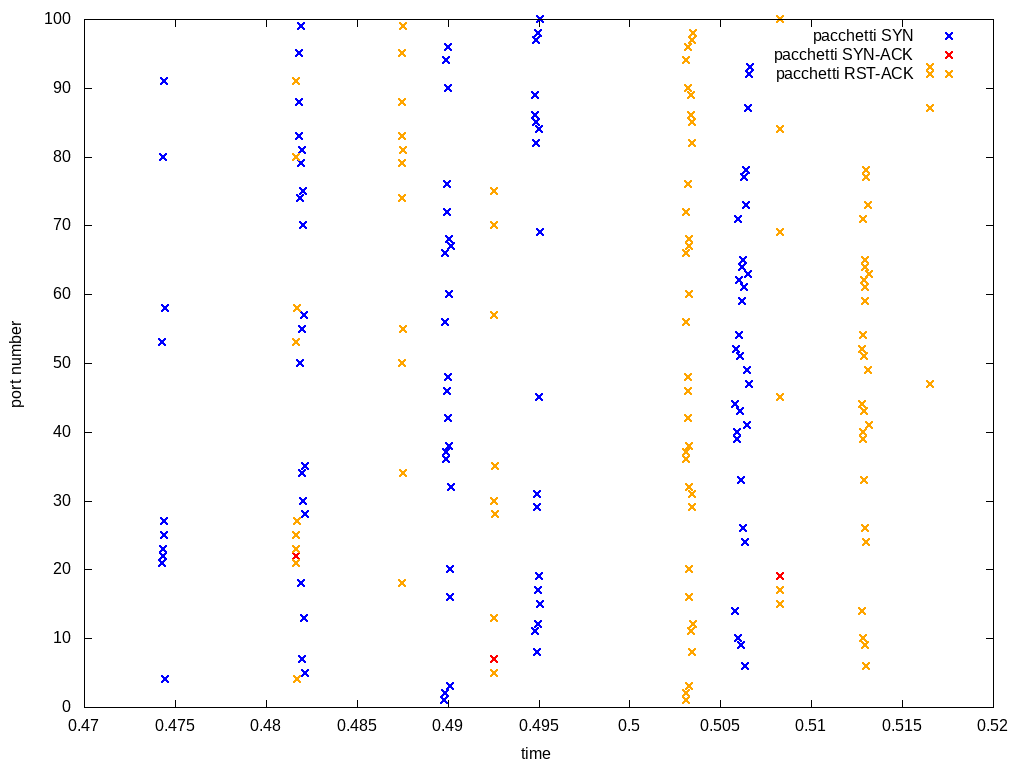
\includegraphics[width=1\linewidth]{vm_tcp_completo.png}
    \vspace{-5pt}
    \caption{TCP scan}\label{Fig:tcp1}
  \end{minipage}%
  \begin{minipage}{0.49\textwidth}
    \centering
    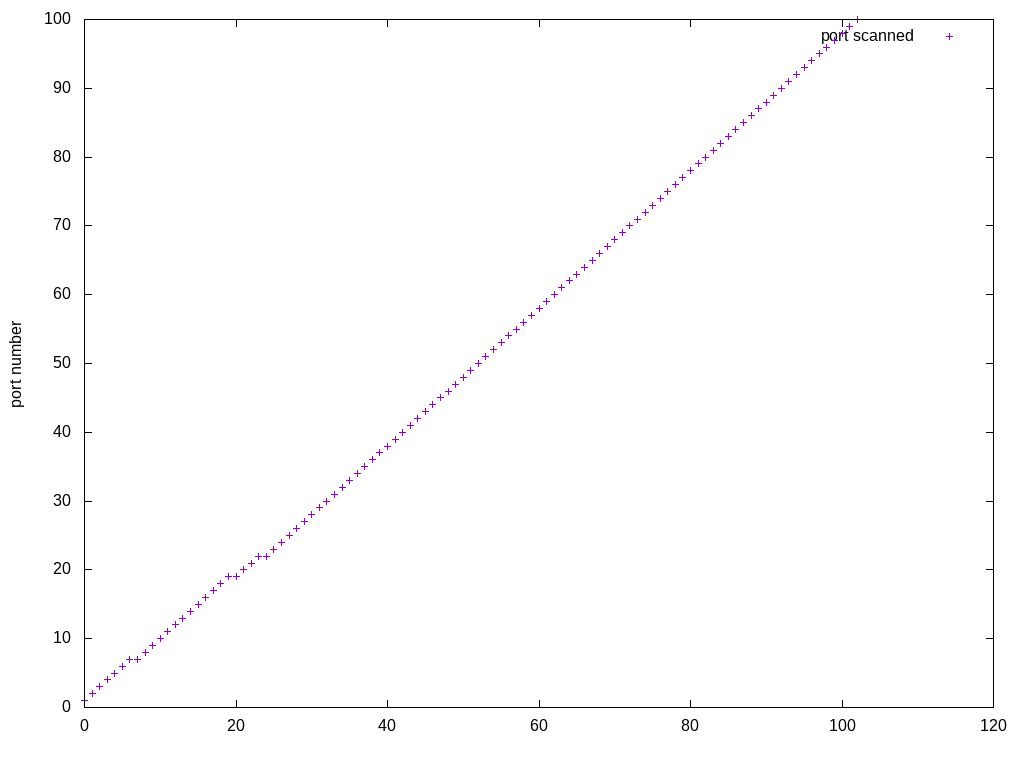
\includegraphics[width=1\linewidth]{vm_tcp_num_test.png}
    \vspace{-5pt}
    \caption{numero di scan per porta}\label{Fig:num}
  \end{minipage}
\end{figure}

\begin{wrapfigure}{l}{0.5\textwidth} %this figure will be at the right
  \centering
  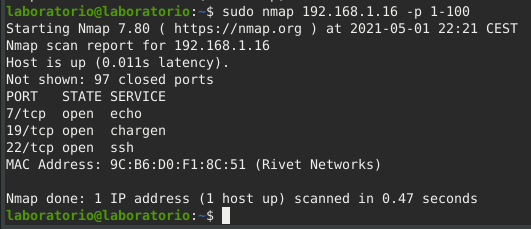
\includegraphics[width=0.5\textwidth]{servizi attivi su vm.png}
  \vspace{-10pt}
\end{wrapfigure}%
\pagebreak
Lo scan delle porte TCP ha richiesto 0.47 secondi complessivamente, ed il tempo
per mandare i singoli pacchetti TCP è anche minore. Per rendere meno evidente 
l'invio di pacchetti quasi simultaneo verso un singolo host, è importante
notare l'ordine delle porte con cui viene eseguito il comando (Figura 3):
le prime ad essere interrogate sono le \textit{well-known port} presenti nel range di porte specificato,
 poichè solitamente più utilizzate; la lista delle porte rimanenti è poi attraversato
 in maniera casuale. Dalla Figura 4 si nota che ogni porta è interrogata una singola volta, poichè TCP 
 è un protocollo affidabile e \textit{connection-oriented}. I pacchetti duplicati che si vedono dal grafico sono 
 i pacchetti di RST mandati dalla sorgente per chiudere le connessioni attive, che corrispondono alle porte 
 aperte trovate [7-19-22] visibili anche in Figura 3. 

 \subsection{Scan UDP}
 Il comando $$sudo\; nmap \;192.168.1.16\; -p \; 1-100 \; -sU$$ permette di eseguire lo scan delle prime 100 porte 
 utilizzando il protocollo UDP. Per comprendere il comportamento del comando con questa
 ulteriore opzione è importante tenere a mente che UDP è un protocollo \textit{connectionless}
 e \textit{best-effort}. Per questo motivo l'invio di un pacchetto UDP può portare a 3 scenari indistinguibili 
 dal lato del mittente:
 \begin{itemize}
  \item[-] la destinazione non risponde
  \vspace{-5pt} 
  \item[-] la porta è filtrata
  \vspace{-5pt}
  \item[-] il pacchetto è andato perso
\end{itemize}

 \begin{figure}[!htb]
  \begin{minipage}{0.49\textwidth}
    \centering
    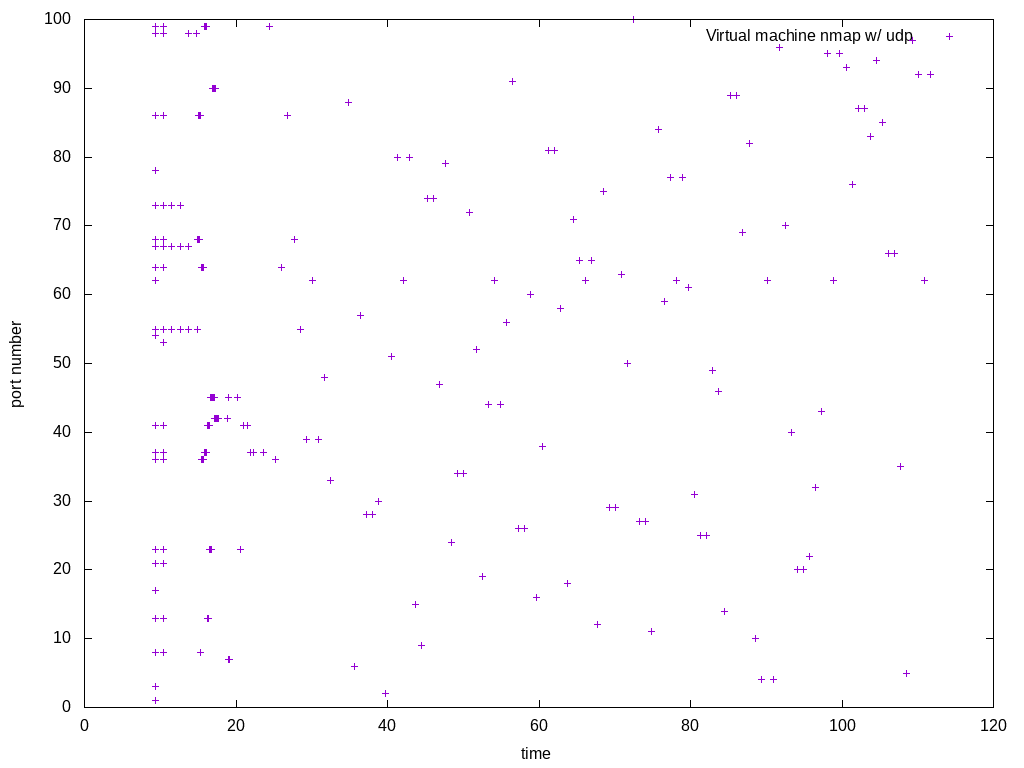
\includegraphics[width=1\linewidth]{vm_udp.png}
    \vspace{-10pt}
    \caption{UDP scan}\label{Fig:tcp2}
  \end{minipage}\hfill
  \begin{minipage}{0.49\textwidth}
    \centering
    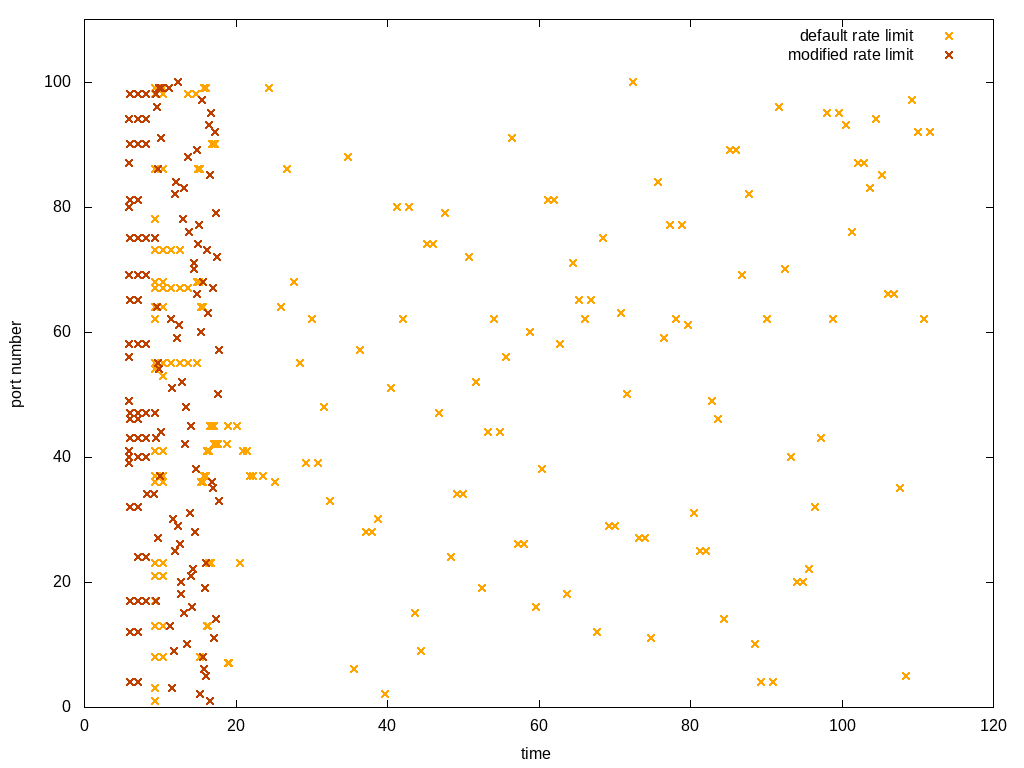
\includegraphics[width=1\textwidth]{ratelimit.png}
    \vspace{-10pt}
    \caption{Modifiche a ICMP port unreach. ratelimit}\label{Fig:ratelimit}
    
  \end{minipage}
\end{figure}

\begin{wrapfigure}{l}{0.5\textwidth} %this figure will be at the right
  \centering
  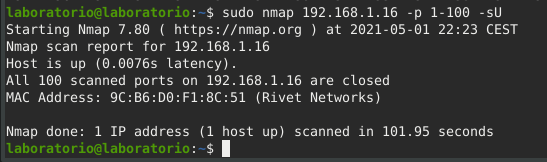
\includegraphics[width=0.5\textwidth]{Servizi attivi su vm con udp.png}
\end{wrapfigure}

L'informazione fondamentale da notare è il tempo di esecuzione: per terminare
il comando impiega 101.95 secondi, di molto superiore al tempo di esecuzione 
per lo scan TCP. Il motivo principale è riconducibile al tentativo del sistema 
operativo di limitare le risposte \textit{ICMP port unreachable}, poprio per 
rendere il port scanning più oneroso in termini di tempo. In particolare 
l'informazione è un valore intero espresso in millisecondi, impostato di
default al valore 1000 (1 secondo) salvato in \textit{/proc/sys/net/ipv4/icmp\_ratelimit}. Questo valore è modificabile con 
il seguente comando: $sudo\; sysctl\; -w\; net.ipv4.icmp\_ratelimit\;=\;10$, che imposta 
il limite delle risposte a 1 ogni 10\textit{ms}. La differenza tra i 
tempi impiegati è apprezzabile nel grafico in Figura 6. \\

\begin{wrapfigure}{r}{0.5\textwidth} %this figure will be at the right
  \centering
  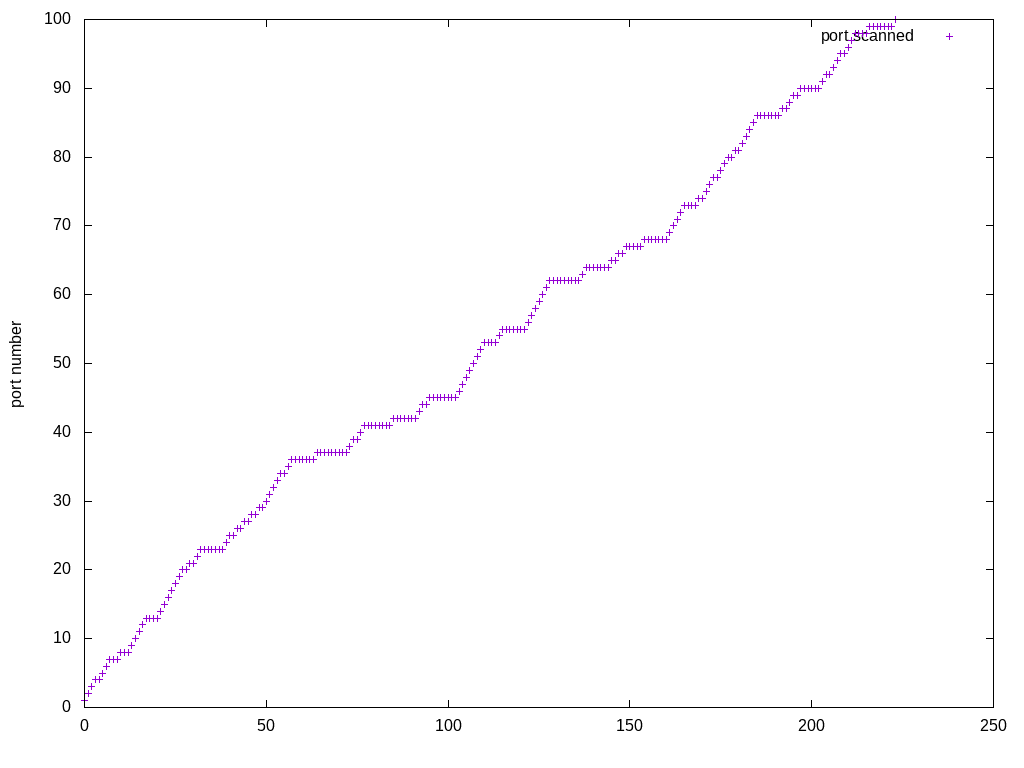
\includegraphics[width=1\linewidth]{vm_udp_num_test.png}  
  \caption{numero di scan per porta}\label{Fig:num2}
\end{wrapfigure}

In figura 7 è possibile notare l'altra grande differenza con uno scan TCP.
Essendo UDP \textit{best-effort} non è sufficiente interrogare la porta una
sola volta. Prima di marcare la porta come filtrata (protetta da un firewall)
o chiusa vengono fatti diversi tentativi. Uno dei motivi per cui i pacchetti 
sonda UDP sono scartati è la loro composizione: la maggior parte di questi viene
mandata come pacchetto privo di payload, il quale viene marcato come non valido 
dal ricevitore anche se la porta UDP è aperta, poichè non è conforme ai pacchetti 
che si aspetta di ricevere. Dal grafico in Figura 5 è possibile inoltre notare 
come UDP si adatti alla rete. Inizialmente infatti vengono mandati diversi pacchetti ma,
non appena il protocollo si accorge di stare inondando la rete con pacchetti che la destinazione 
scarterebbe avendo già raggiunto il limite di ICMP port unreachable discusso precedentemente, 
adatta la propria velcità a tale limite. 

\section{Analisi delle prime 100 porte della Firestick TV}
\subsection{Scan TCP}
\begin{figure}[!htb]
  \begin{minipage}{0.49\textwidth}
    \centering
    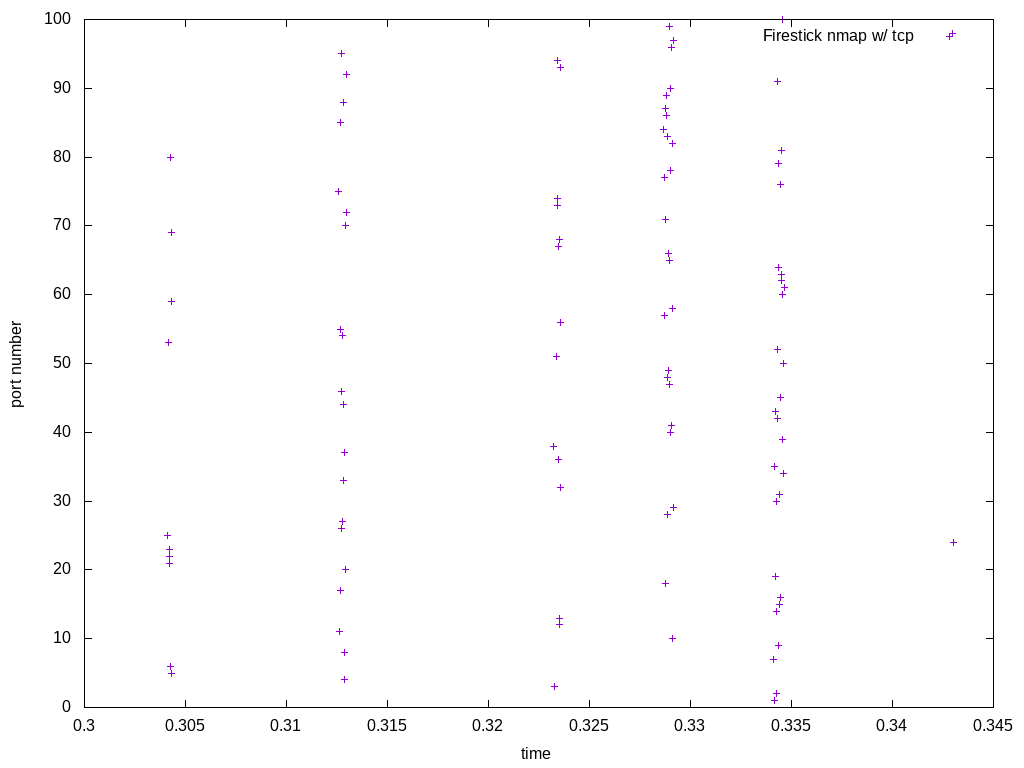
\includegraphics[width=1\linewidth]{firestick_tcp.png}
    \vspace{-5pt}
    \caption{TCP scan}\label{Fig:tcp3}
  \end{minipage}\hfill
  \begin{minipage}{0.49\textwidth}
    \centering
    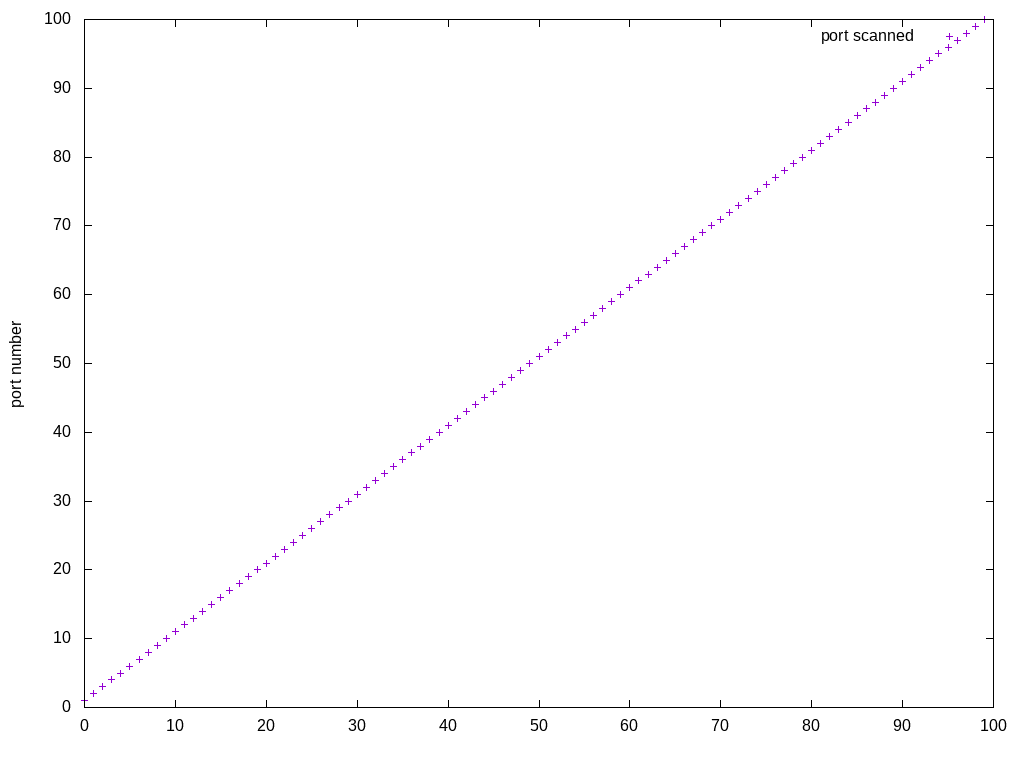
\includegraphics[width=1\linewidth]{Firestick_tcp_num_test.png}
    \vspace{-5pt}
    \caption{numero di scan per porta}\label{Fig:num3}
  \end{minipage}
\end{figure}
Eseguendo il comando  $sudo\; nmap \;192.168.1.11\; -p \; 1-100$ si esegue lo scan tcp delle 
prime 100 porte dell'host indicato. Dal grafico in Figura 8 è possibile avere conferma delle 
considerazioni fatte al caso precedente. Questa modalità di \textit{host-discovery} e scan è particolarmente
efficiente, è possibile infatti notare come vengano mandati tutti e 100 pacchetti TCP SYN in alcune decine 
di millisecondi. I primi pacchetti ad essere mandati hanno nuovamente come destinazione le 
\textit{well-known} port nel range specificato, che ospitano servizi quali ECHO, FTP, SSH, SMTP, DNS, HTTP\dots \\
Queste porte vengono privilegiate per rendere la scansione più rapida: se l'host dovesse essere attivo è più probabile
che abbia queste porte aperte; in questo modo si può dire rapidamente se l'host è attivo, evitando di mandare inutilmente 
pacchetti in rete. 


In Figura 9 è possibile notare il numero di tentativi per porta eseguiti da nmap, che restano costanti 
al valore 1, non essendoci servizi aperti sull'host ed essendo TCP affidabile e \textit{connection-orentied}. 
Un particolare degno di nota è che con questo tipo di scansione non sempre tutte le porte aperte vengono rilevate,
principalmente per la presenza di firewall, mentre eseguendo una scnasione più completa risulata aperta su questo dispositivo
la porta TCP 8009, che ospita il servizio "ajp13", vulnerabile a LFI (Local File Inclusion).







\subsection{Scan UDP}
\begin{figure}[!htb]
  \begin{minipage}{0.49\textwidth}
    \centering
    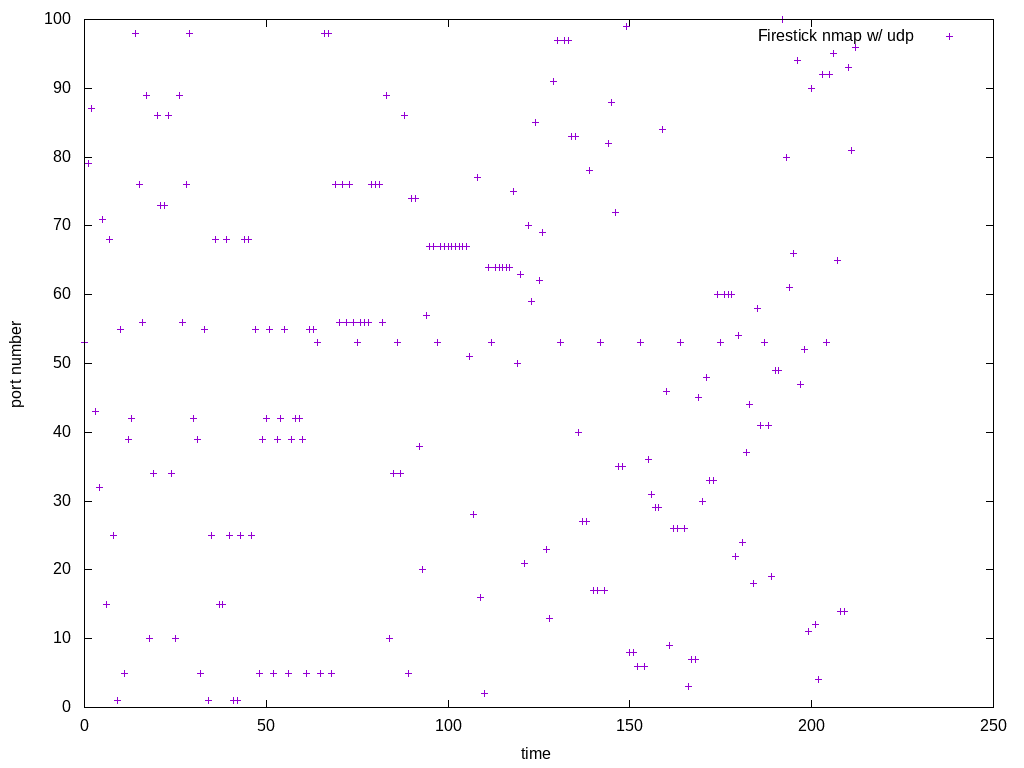
\includegraphics[width=1\linewidth]{Firestick_udp.png}
    \vspace{-10pt}
    \caption{UDP scan}\label{Fig:tcp4}
  \end{minipage}\hfill
  \begin{minipage}{0.49\textwidth}
    \centering
    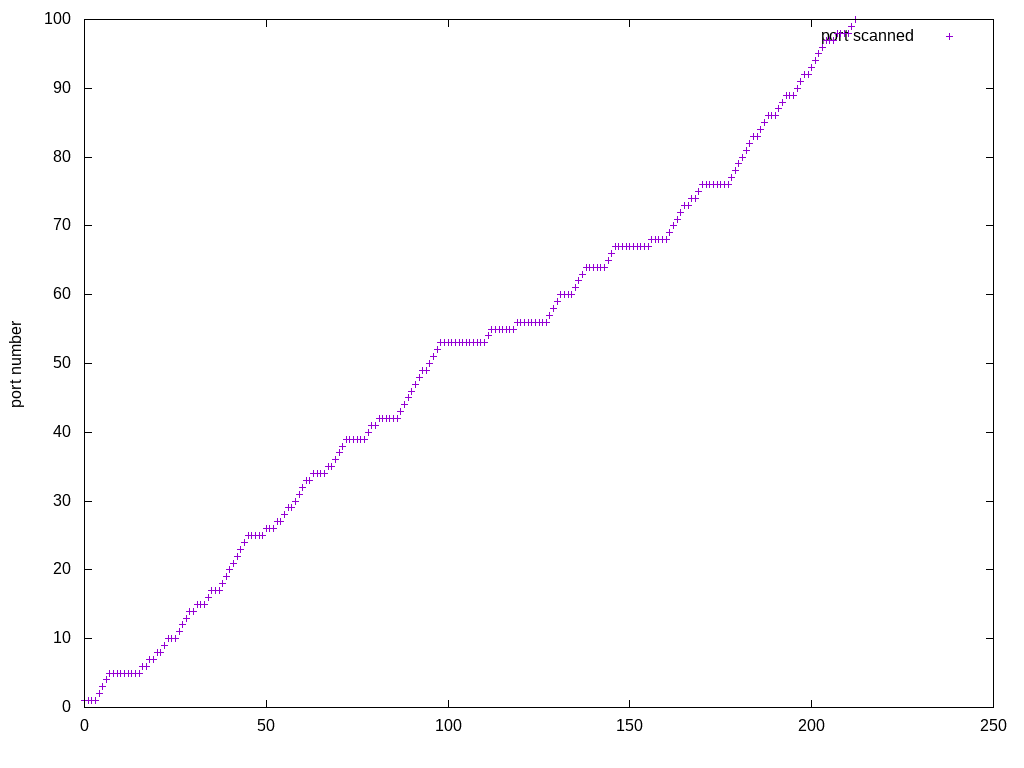
\includegraphics[width=1\textwidth]{Firestick_udp_num_test.png}
    \vspace{-10pt}
    \caption{Numero di scan per porta}\label{Fig:scan}
    
  \end{minipage}
\end{figure}
Eseguendo il comando $sudo\; nmap \;192.168.1.11\; -p \; 1-100 \; -sU$ si ottiene anche in questo caso conferma dei ragionamenti 
fatti in precedenza per uno scan UDP. Non essendo noti con certezza il sistema operativo dell'host, e di conseguenza il suo 
comportamento in risposta ai \textit{probe} UDP, si può solo evidenziare come in questo caso rispetto al precedente ci metta più tempo
ad adattarsi ai limiti imposti alla destinazione, evitando \textit{flood} della rete. Infatti se nel primo caso come si nota in Figura 5
il transitorio verso la fase in cui il mittente è allineato con le capacità di risposta del destinatario (limitate dalla rete o da altri fattori come visto nel punto 1.2)
dura una decina di secondi, in questo secondo caso si risolve parzialmente solo a metà scan, come si può evincere dalla Figura 10, vista la densità di 
pacchetti nella prima metà dello scan. \\
\begin{wrapfigure}{l}{0.5\textwidth} %this figure will be at the right
  \centering
  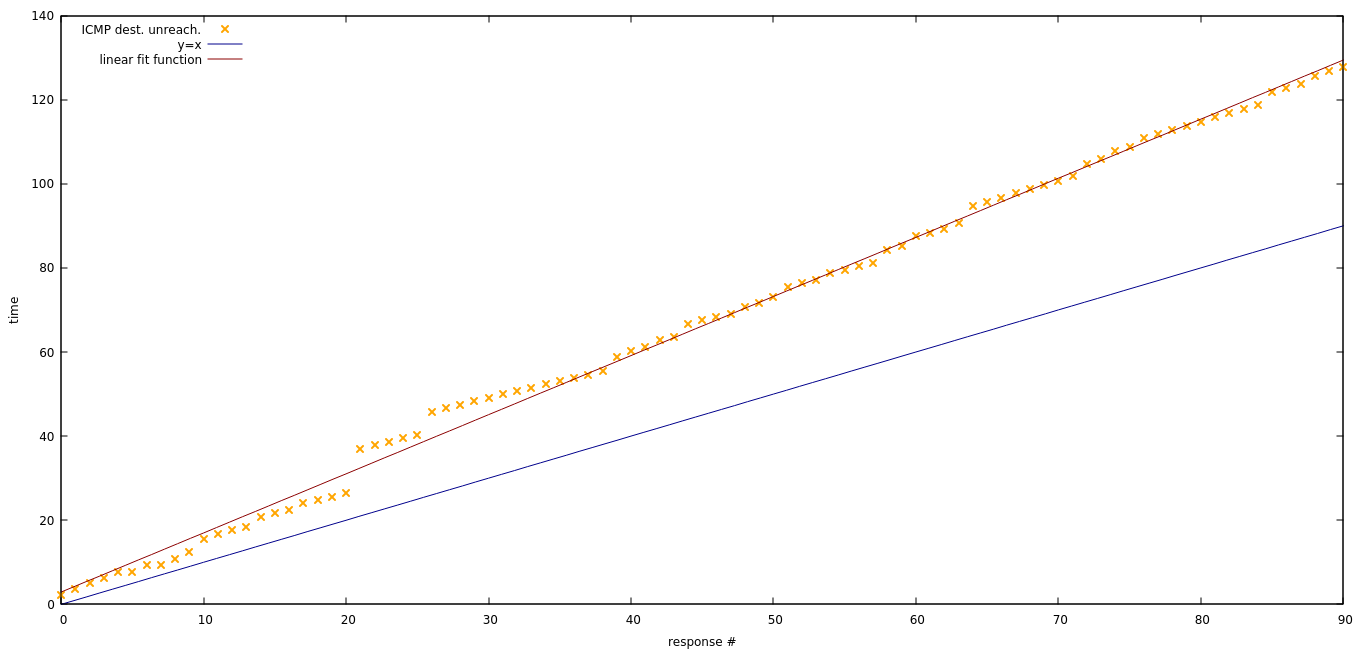
\includegraphics[width=0.5\textwidth]{port_unreach_vs_time (1).png}
  \caption{ICMP destination unreachable}\label{Fig:icmp}
\end{wrapfigure}
\'E inoltre possibile notare che la quantità di pacchetti mandati e il tempo impiegato per mandarli (e di conseguenza ricevere i messaggi
ICMP in risposta) è praticamente analogo al caso esaminato precedentemente. Questo fa supporre un comportamento simile del sistema operativo per 
limitare il port scanning. In figura 12 è possibile vedere i pacchetti \textit{ICMP destination unreachable} mandati dalla vittima. Se non ci 
fossero intervalli di tempo in cui l'host non ha mandato alcun pacchetto in risposta, l'andamento avrebbe meglio rispecchiato una retta parallela ad $y(t)=x(t)$,
una relazione lineare che fa corrispondere ad ogni secondo un singolo pacchetto mandato dalla vittima in risposta al \textit{probe}. 



\pagebreak
\section{Appendice}
\subsection{Script per preparazione dataset}
        \begin{verbatim}
          #!/bin/bash

          final=$(echo "$1" | cut -f 1 -d '.')_def.dat
          cat $1 | tr -s ' ' | cut -d ' ' -f 10 > nmap_port.dat
          cat $1 | tr -s ' ' | cut -d ' ' -f 3 > nmap_time.dat
          
          paste nmap_time.dat nmap_port.dat > $final
          
          rm nmap_port.dat
          rm nmap_time.dat
          \end{verbatim}
\subsection{Script per grafico Figura 2}
\subsubsection{Collezione dati}
\begin{verbatim}
  for((s=0; s<100; s+=1))
do
	sudo nmap 192.168.1.1-100  | grep "scanned in" | cut -d ' ' -f11 >> nmap_sudo_time.dat
done
  for((s=0; s<100; s+=1))
do
	nmap 192.168.1.1-100  | grep "scanned in" | cut -d ' ' -f11 >> nmap_time.dat
done

\end{verbatim}
\subsubsection{Grafico}
 \begin{verbatim}
  set xlabel "n° tentativo"
  set ylabel "time"
  set terminal png size 1024, 768
  set output "sudo_vs_normaluser.png"
  
  f(x)=a*x+b
  g(x)=c*x+d
  fit f(x) 'nmap_time.dat' via a,b
  fit g(x) 'nmap_sudo_time.dat' via c,d

  plot 'nmap_time.dat' title "without root permission" lc rgb "orange" pt 2 lw 2,
       'nmap_sudo_time.dat' title "with root permission" lc rgb "dark-red" pt 2 lw 2.5,
       f(x) lc "red",
       g(x) lc "green"
 \end{verbatim}
\subsection{Script per grafici TCP Figura 3}
\begin{verbatim}
  set xlabel "time"
  set ylabel "port number"
  set terminal png size 1024, 768
  set output "vm_tcp.png"
  
  plot  'nmap_syn_def.dat' using 1:2 title "pacchetti SYN" lc rgb "blue" pt 2 lw 2,
    'nmap_synack_def.dat' using 1:2 title "pacchetti SYN-ACK" lc rgb "red" pt 2 lw 2.5,
    'nmap_rstack_def.dat' using 1:2 title "pacchetti RST-ACK" lc rgb "orange" pt 2 lw 2 
\end{verbatim}
\subsection{Script per grafici Figura 8, 9, 10, 11 e simili}
\begin{verbatim}
set terminal png size 1024, 768

set xlabel "time"
set ylabel "port number"
set output "firestick_tcp.png"
plot 'nmap_def.dat' using 1:2 title "Firestick nmap w/ tcp" 

set xlabel "time"
set ylabel "port number"
set output "Firestick_udp.png"
plot 'nmap_udp_def.dat' using :2 title "Firestick nmap w/ udp" 

set output "Firestick_tcp_num_test.png"
set ylabel "port number"
plot '<sort -n -k 2 nmap_def.dat' using :2 title "port scanned"

set output "Firestick_udp_num_test.png"
set ylabel "port number"
plot '<sort -n -k 2 nmap_udp_def_dnsecho.dat' using :2 title "port scanned"
\end{verbatim}

\subsection{Script per Figura 12}
\begin{verbatim}
  set xlabel "response #"
  set ylabel "time"
  set terminal png size 1024, 768
  set output "ICMP_d_u.png"
  
  f(x)=a*x+b
  fit f(x) 'icmp_pu.dat' via a,b
  set yrange [0:140]
  set xrange [0:90]

  plot 'icmp_pu.dat' title "ICMP dest. unreach." lc rgb "orange" pt 2 lw 2,
       x lc "dark-blue" title "y=x",
       f(x) lc "dark-red" title "linear fit function"
\end{verbatim}
\pagebreak
\subsection{Log file dei fit}
\subsubsection{fit nello script al punto 3.5}
\begin{verbatim}
      *******************************************************************************
      Sun May  9 00:53:17 2021


      FIT:    data read from 'data.dat'
              format = z
              #datapoints = 92
              residuals are weighted equally (unit weight)

      function used for fitting: f(x)
        f(x) = a*x+b
      fitted parameters initialized with current variable values

      iter      chisq       delta/lim  lambda   a             b            
        0 4.9279558493e+04   0.00e+00  3.73e+01    1.000000e+00   1.000000e+00
        4 4.1866803645e+02  -9.63e-02  3.73e-03    1.405480e+00   2.925743e+00

      After 4 iterations the fit converged.
      final sum of squares of residuals : 418.668
      rel. change during last iteration : -9.62567e-07

      degrees of freedom    (FIT_NDF)                        : 90
      rms of residuals      (FIT_STDFIT) = sqrt(WSSR/ndf)    : 2.15682
      variance of residuals (reduced chisquare) = WSSR/ndf   : 4.65187

      Final set of parameters            Asymptotic Standard Error
      =======================            ==========================
      a               = 1.40548          +/- 0.008467     (0.6025%)
      b               = 2.92574          +/- 0.4461       (15.25%)

      correlation matrix of the fit parameters:
                      a      b      
      a               1.000 
      b              -0.864  1.000 
\end{verbatim}
\subsubsection{fit nello script al punto 3.2.2}
\begin{verbatim}
      *******************************************************************************
      Sat May  8 00:50:24 2021
      
      
      FIT:    data read from 'nmap_sudo_time.dat'
              format = z
              #datapoints = 100
              residuals are weighted equally (unit weight)
      
      function used for fitting: f(x)
        f(x)=a*x+b
      fitted parameters initialized with current variable values
      
      iter      chisq       delta/lim  lambda   a             b            
        0 3.3359392660e+05   0.00e+00  4.05e+01    1.000000e+00   1.000000e+00
        5 1.7438891689e+00  -1.17e-08  4.05e-04    6.780678e-04   4.284356e-01
      
      After 5 iterations the fit converged.
      final sum of squares of residuals : 1.74389
      rel. change during last iteration : -1.16886e-13
      
      degrees of freedom    (FIT_NDF)                        : 98
      rms of residuals      (FIT_STDFIT) = sqrt(WSSR/ndf)    : 0.133397
      variance of residuals (reduced chisquare) = WSSR/ndf   : 0.0177948
      
      Final set of parameters            Asymptotic Standard Error
      =======================            ==========================
      a               = 0.000678068      +/- 0.0004621    (68.15%)
      b               = 0.428436         +/- 0.02648      (6.181%)
      
      correlation matrix of the fit parameters:
                      a      b      
      a               1.000 
      b              -0.864  1.000 
      
      
      *******************************************************************************
      Sat May  8 00:50:44 2021
      
      
      FIT:    data read from 'nmap_time.dat'
              format = z
              #datapoints = 100
              residuals are weighted equally (unit weight)
      
      function used for fitting: g(x)
        g(x)=c*x+d
      fitted parameters initialized with current variable values
      
      iter      chisq       delta/lim  lambda   c             d            
        0 3.3733228500e+05   0.00e+00  4.05e+01    1.000000e+00   1.000000e+00
        5 1.8316262826e-02  -2.75e-06  4.05e-04   -1.411341e-04   1.101861e-01
      
      After 5 iterations the fit converged.
      final sum of squares of residuals : 0.0183163
      rel. change during last iteration : -2.7494e-11
      
      degrees of freedom    (FIT_NDF)                        : 98
      rms of residuals      (FIT_STDFIT) = sqrt(WSSR/ndf)    : 0.0136712
      variance of residuals (reduced chisquare) = WSSR/ndf   : 0.000186901
      
      Final set of parameters            Asymptotic Standard Error
      =======================            ==========================
      c               = -0.000141134     +/- 4.736e-05    (33.56%)
      d               = 0.110186         +/- 0.002714     (2.463%)
      
      correlation matrix of the fit parameters:
                      c      d      
      c               1.000 
      d              -0.864  1.000   
\end{verbatim}




























\end{document}
\begin{flushleft}
  Eseguiamo il comando: ping 10.0.21.31 -b, aggiungendo l’opzione -b per permettere il ping al broadcast.
\end{flushleft}

%\hspace{1.2cm}
\begin{wrapfigure}{r}{0.5\textwidth} %this figure will be at the right
    \centering
    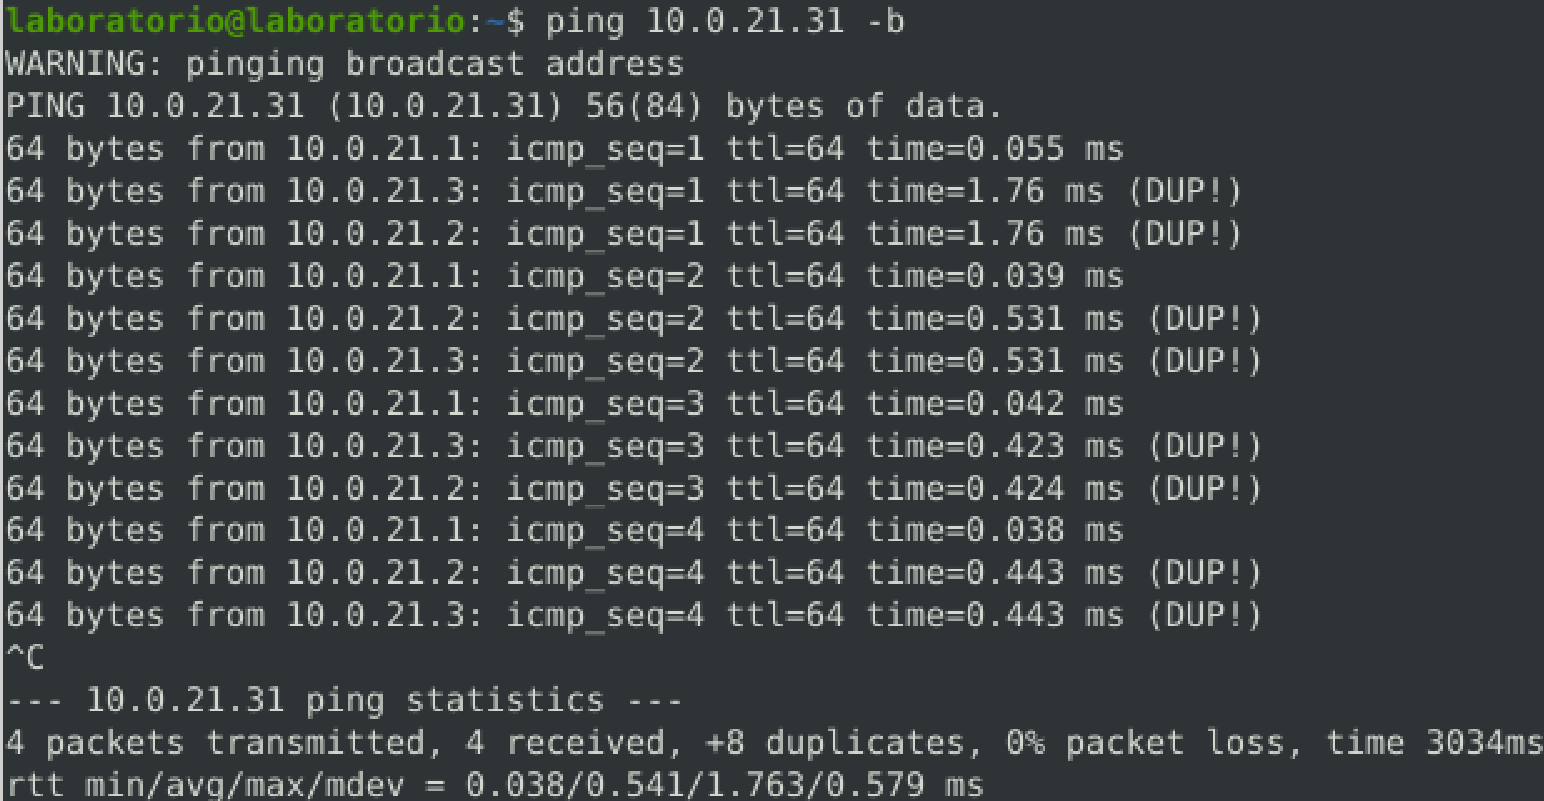
\includegraphics[width=0.5\textwidth]{broadcast1.png}
    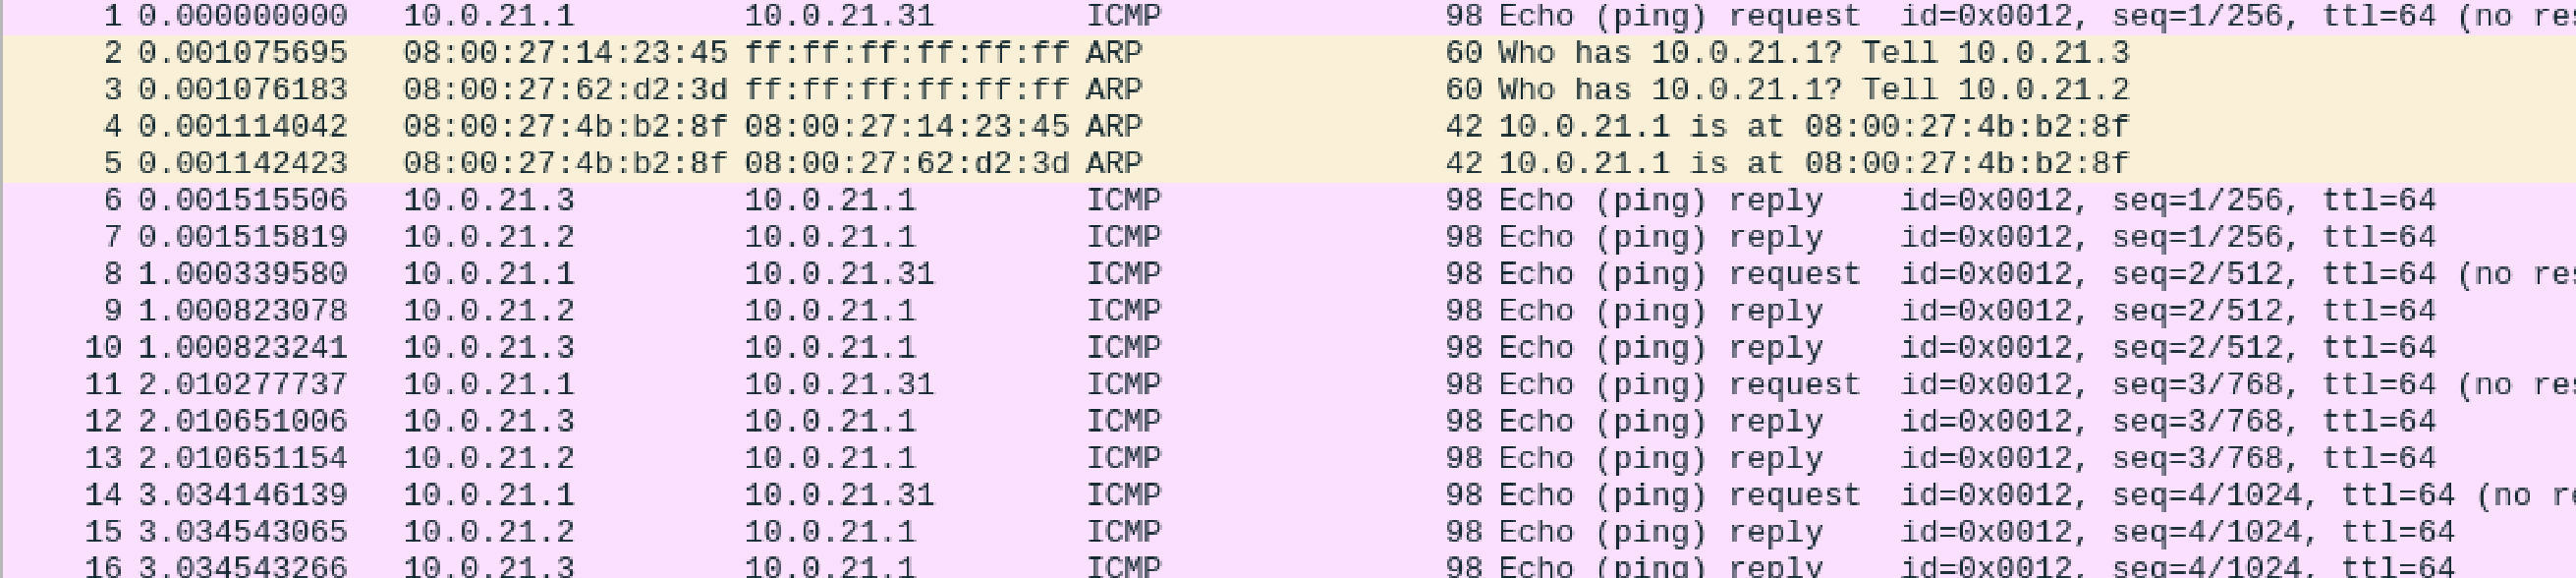
\includegraphics[width=0.5\textwidth]{wiresharkbroadcast.png}
\end{wrapfigure}
\'E
Si può notare che: \\
La prima risposta ricevuta è quella dell’interfaccia di loopback dell’host che effettua il ping. 
Quest'ultima è infatti molto più veloce delle altre, che saranno contrassegnate come duplicate, \textit{"DUP!"}, poiché è già arrivata una risposta al pacchetto con la stessa \textit{icmp\_seq}. 
Queste risposte sono fornite dagli altri host e impiegheranno più tempo ad arrivare a causa della necessità di attraversare il mezzo fisico; 
inoltre il primo pacchetto avrà un campo \textit{time} più elevato per via dell'intervento del protocollo ARP.


Nel caso del ping ad un indirizzo\hyphenation{broadcast} \hyphenation{Request} broadcast, non ci sarà subito una ARP Request da parte dell’host che ha eseguito il comando, dal momento che l’indirizzo MAC di destinazione è noto (\textit{FF:FF:FF:FF:FF:FF}).
Saranno gli host che devono rispondere a doverla effettuare, poiché ARP non è capace di leggere e trarre informazioni dai pacchetti ICMP.
Ad esempio se l’host che esegue il ping è H1, avrà inizialmente la tabella ARP vuota, saranno H2 e H3 a fare le ARP Request. 
Alla fine la tabella ARP di H1 conterrà le coppie indirizzo IP/MAC di H2 e H3, mentre gli altri due host conterranno solo le informazioni di H1.


Se decidessimo di limitare il numero di pacchetti mandati con l'opzione \textit{-c}, non verrebbero visualizzati gli ultimi due pacchetti duplicati poichè l’applicazione ping attende la prima risposta all’ultimo pacchetto prima di terminare.
\pagebreak
\subsection{Ping a indirizzo di rete}

\hspace{1.2cm}
\begin{wrapfigure}{r}{0.8\textwidth} %this figure will be at the right
    \centering
    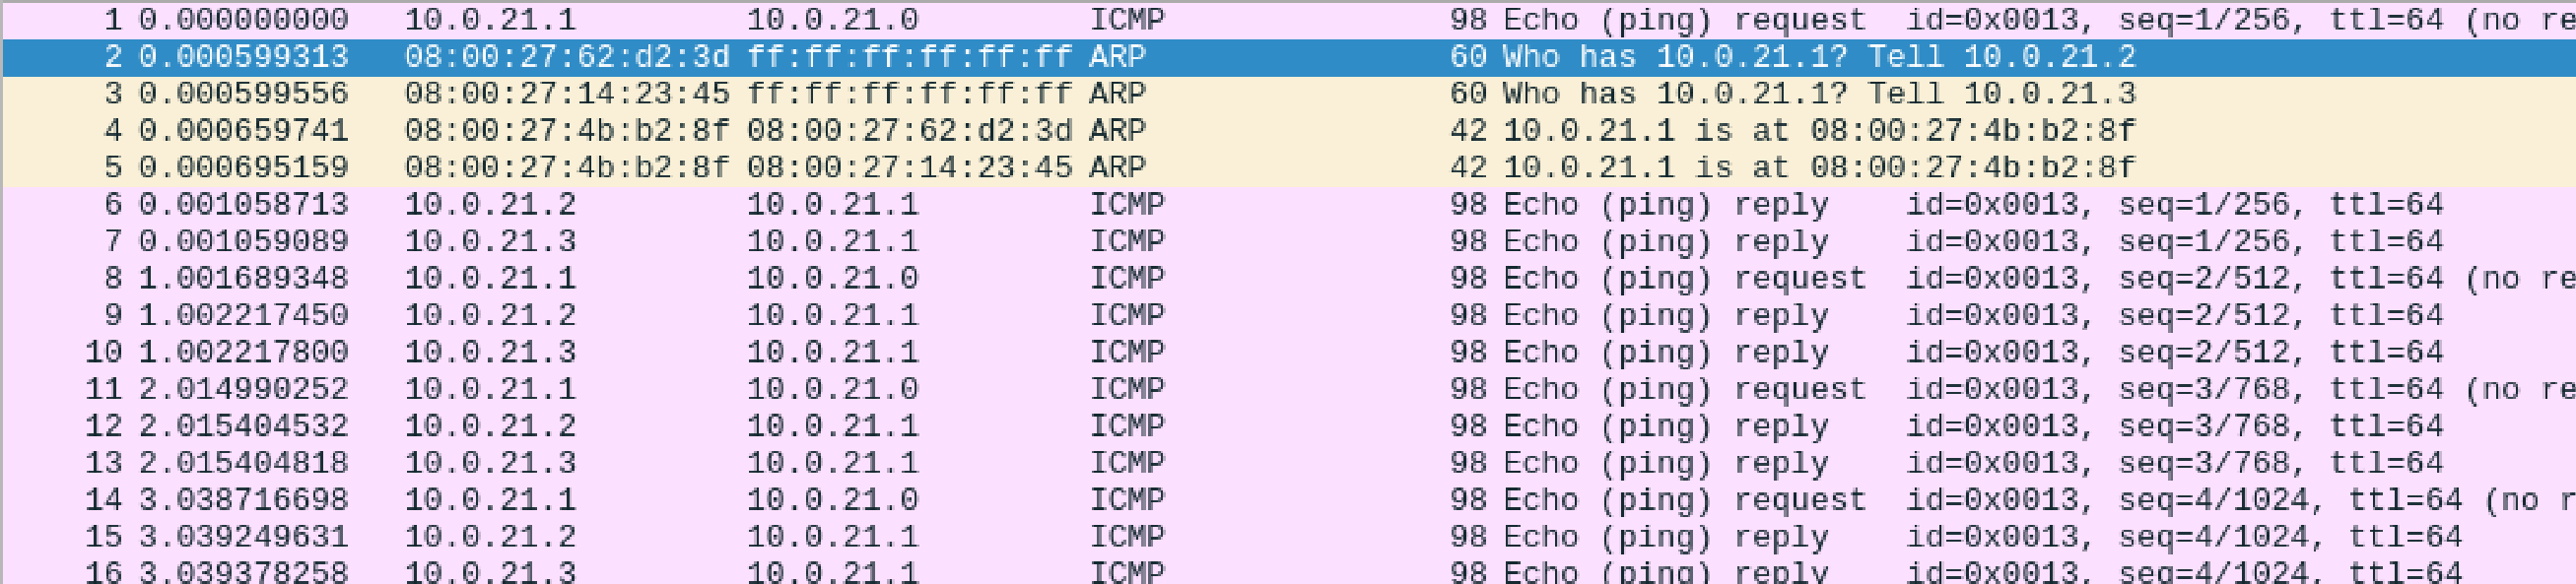
\includegraphics[width=0.7\textwidth]{indirizzorete.png}
\end{wrapfigure}

Si può notare come il comportamento quando si esegue il ping verso l’indirizzo di rete sia identico a quello analizzato quando si esegue il ping all’indirizzo broadcast.

\section{Indirizzi duplicati}

Abbiamo configurato la rete in modo che l’indirizzo ip degli host H1 e H3 sia uguale a 10.0.21.1/27

\subsection{Ping da H2 a H1}

%\hspace{1cm}
\begin{wrapfigure}{r}{0.66\textwidth} %this figure will be at the right
 \vspace{-10pt}
    \centering
    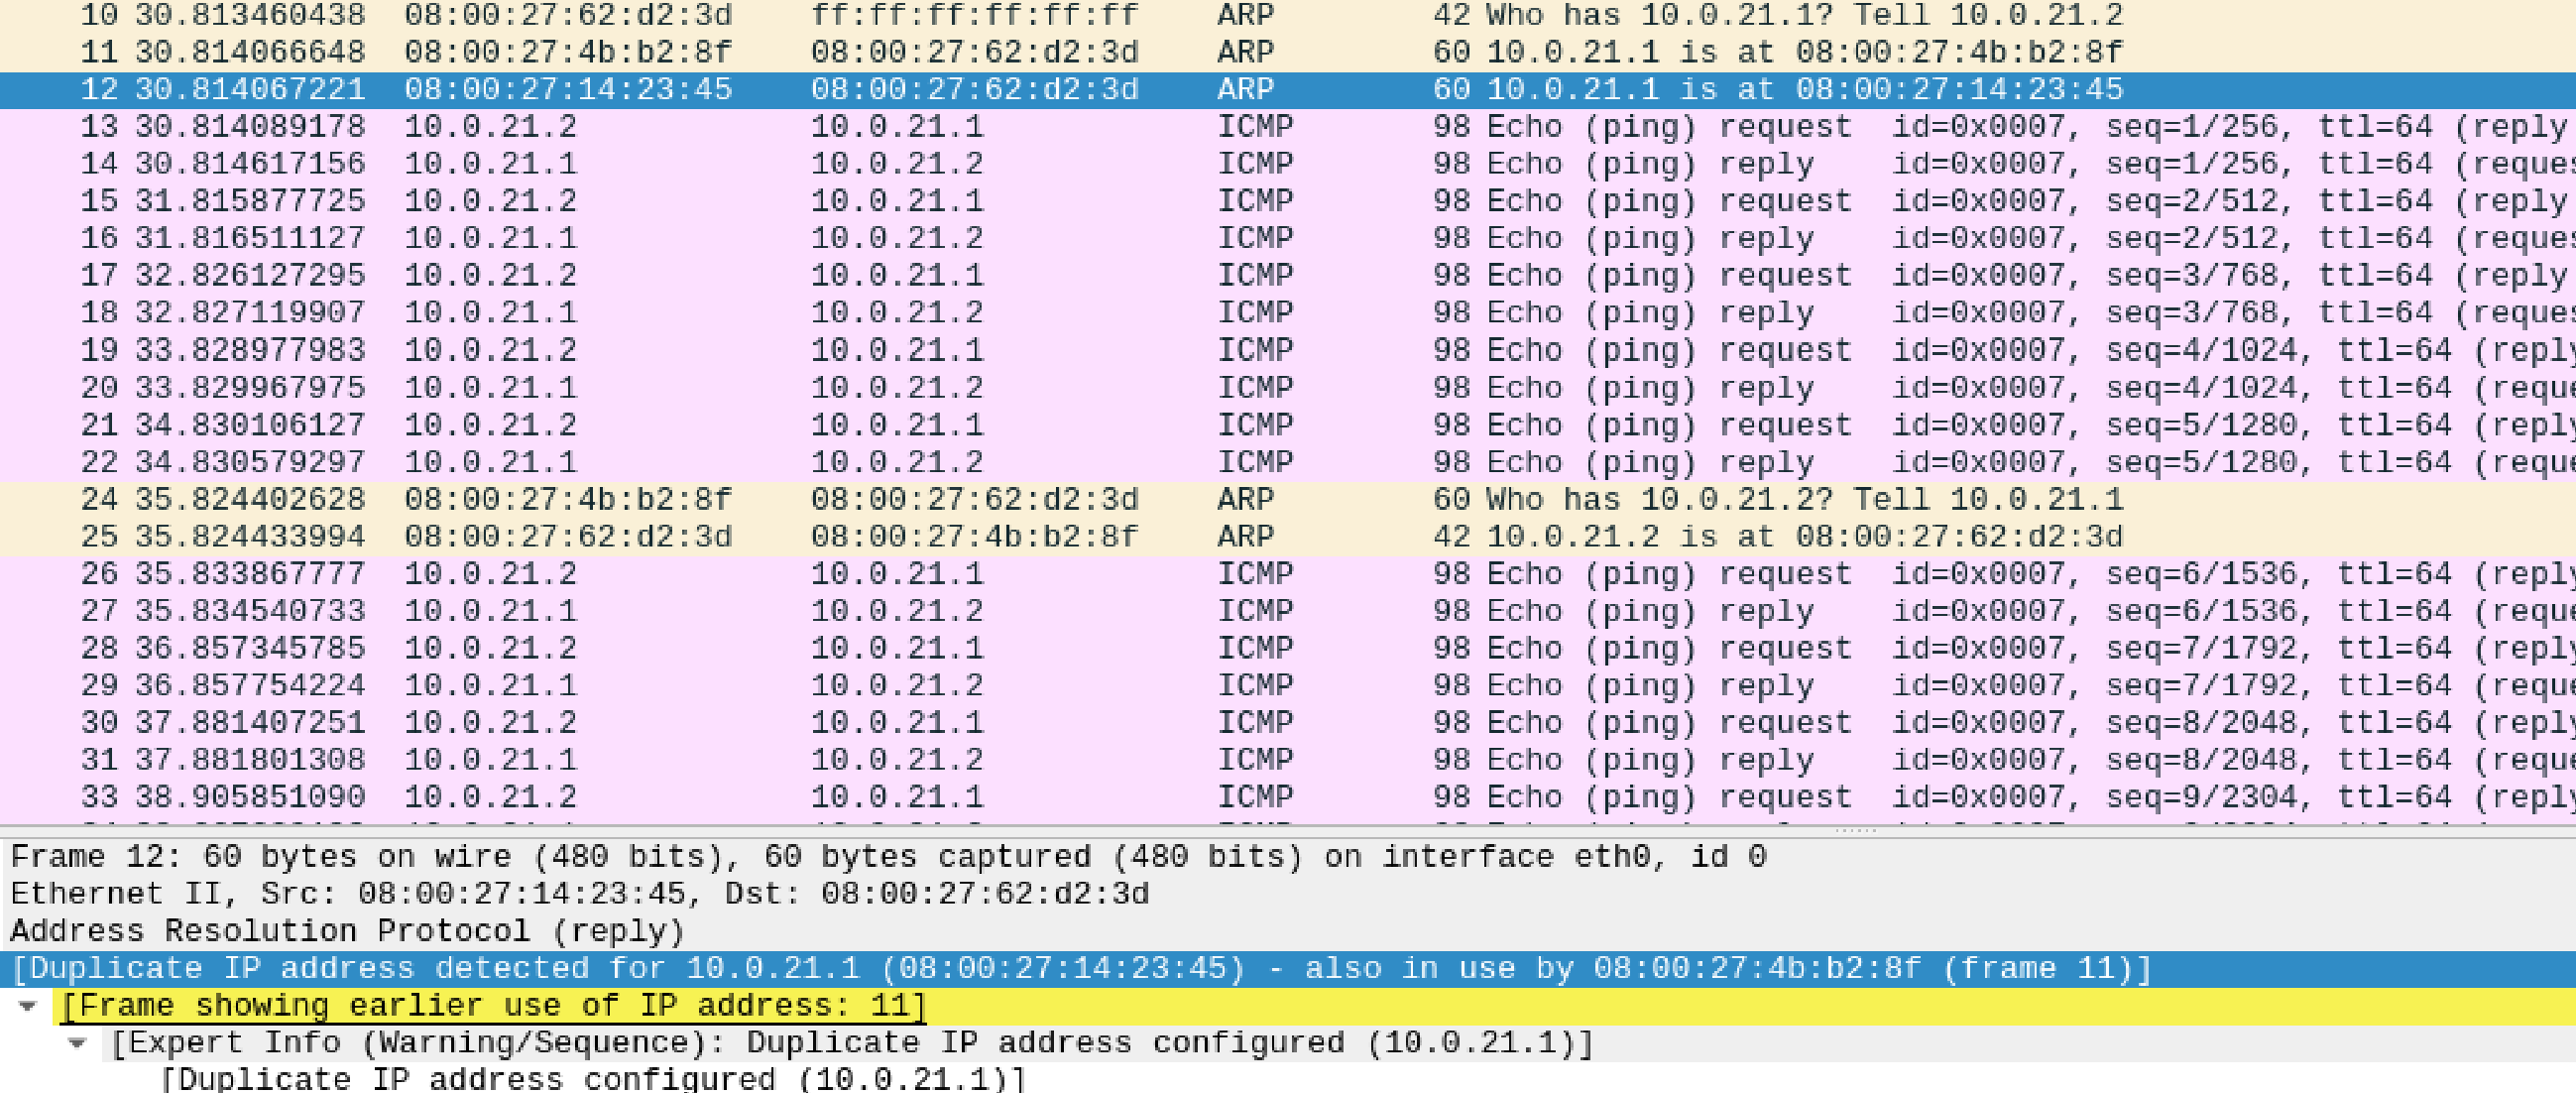
\includegraphics[width=0.6\textwidth]{duplicati1.png}
    \vspace{-5pt}
    \caption{elenco pacchetti in transito su H1}
   
% \end{wrapfigure}
\rule[5mm]{10cm}{0.5pt}
%\rule[5mm]{0mm}{0.5cm}
%\rule{8cm}{0.8pt}
% \begin{wrapfigure}{r}{0.66\textwidth} %this figure will be at the right
  \centering
  \vspace{-5pt}
  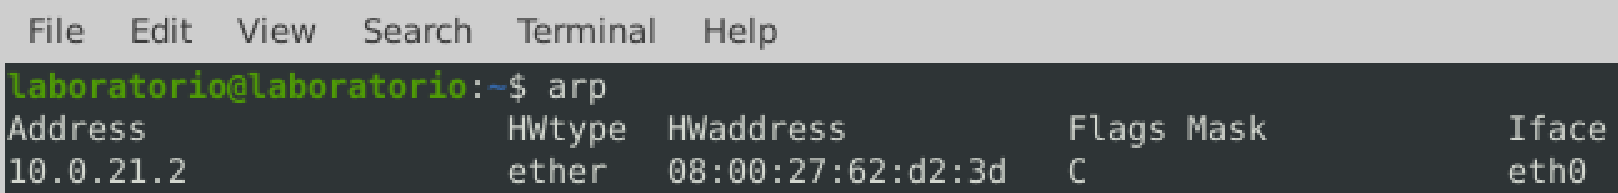
\includegraphics[width=0.6\textwidth]{host1ARP.png}
  \vspace{-4pt}
  \caption{host1}
  \vspace{-20pt}
\end{wrapfigure}
% \begin{figure}
%     \begin{minipage}{0.67\textwidth}
%       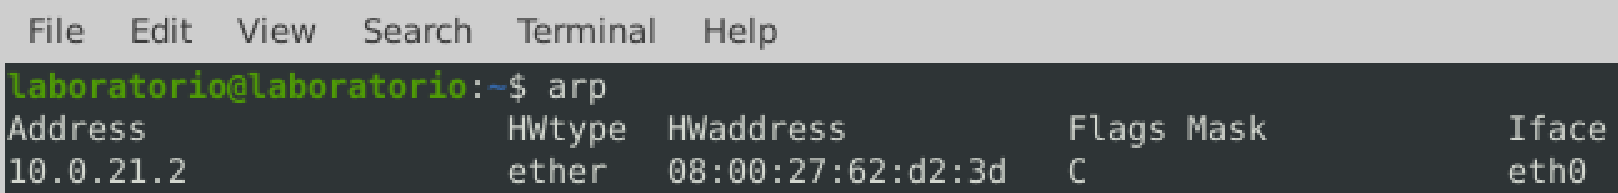
\includegraphics[width=\textwidth]{host1ARP.png}
%     \end{minipage}\hfill
%     \begin{minipage}{0.3\textwidth}
%       \caption{
%          host 1
%       } \label{fig:03-03}
%     \end{minipage}
%   \end{figure}

Se eseguo il ping da H2 verso l’ip 10.0.21.1, wireshark catturerà l’ARP request di H2 e le due ARP reply da parte di H3 e H1. ARP considera solo la prima risposta e marcherà la seconda come \textit{duplicate ip address}, quindi il primo tra H3 e H1 riceverà due \textit{ARP Reply}, mentre il secondo non riceverà nulla.
Come si può notare il rinfresco delle tabelle ARP non viene eseguito tramite un messaggio broadcast, ma viene usato l’indirizzo MAC già presente precedentemente nell'ARP Table. Ad esempio nel nostro caso, la comunicazione avviene solo tra H2 e H1.


\vspace{2cm}
\subsection{Ping da H1 e H3 a H2}



%\hspace{1.2cm}
\begin{wrapfigure}{r}{0.75\textwidth} %this figure will be at the right
  \vspace{-10pt}
    \centering
      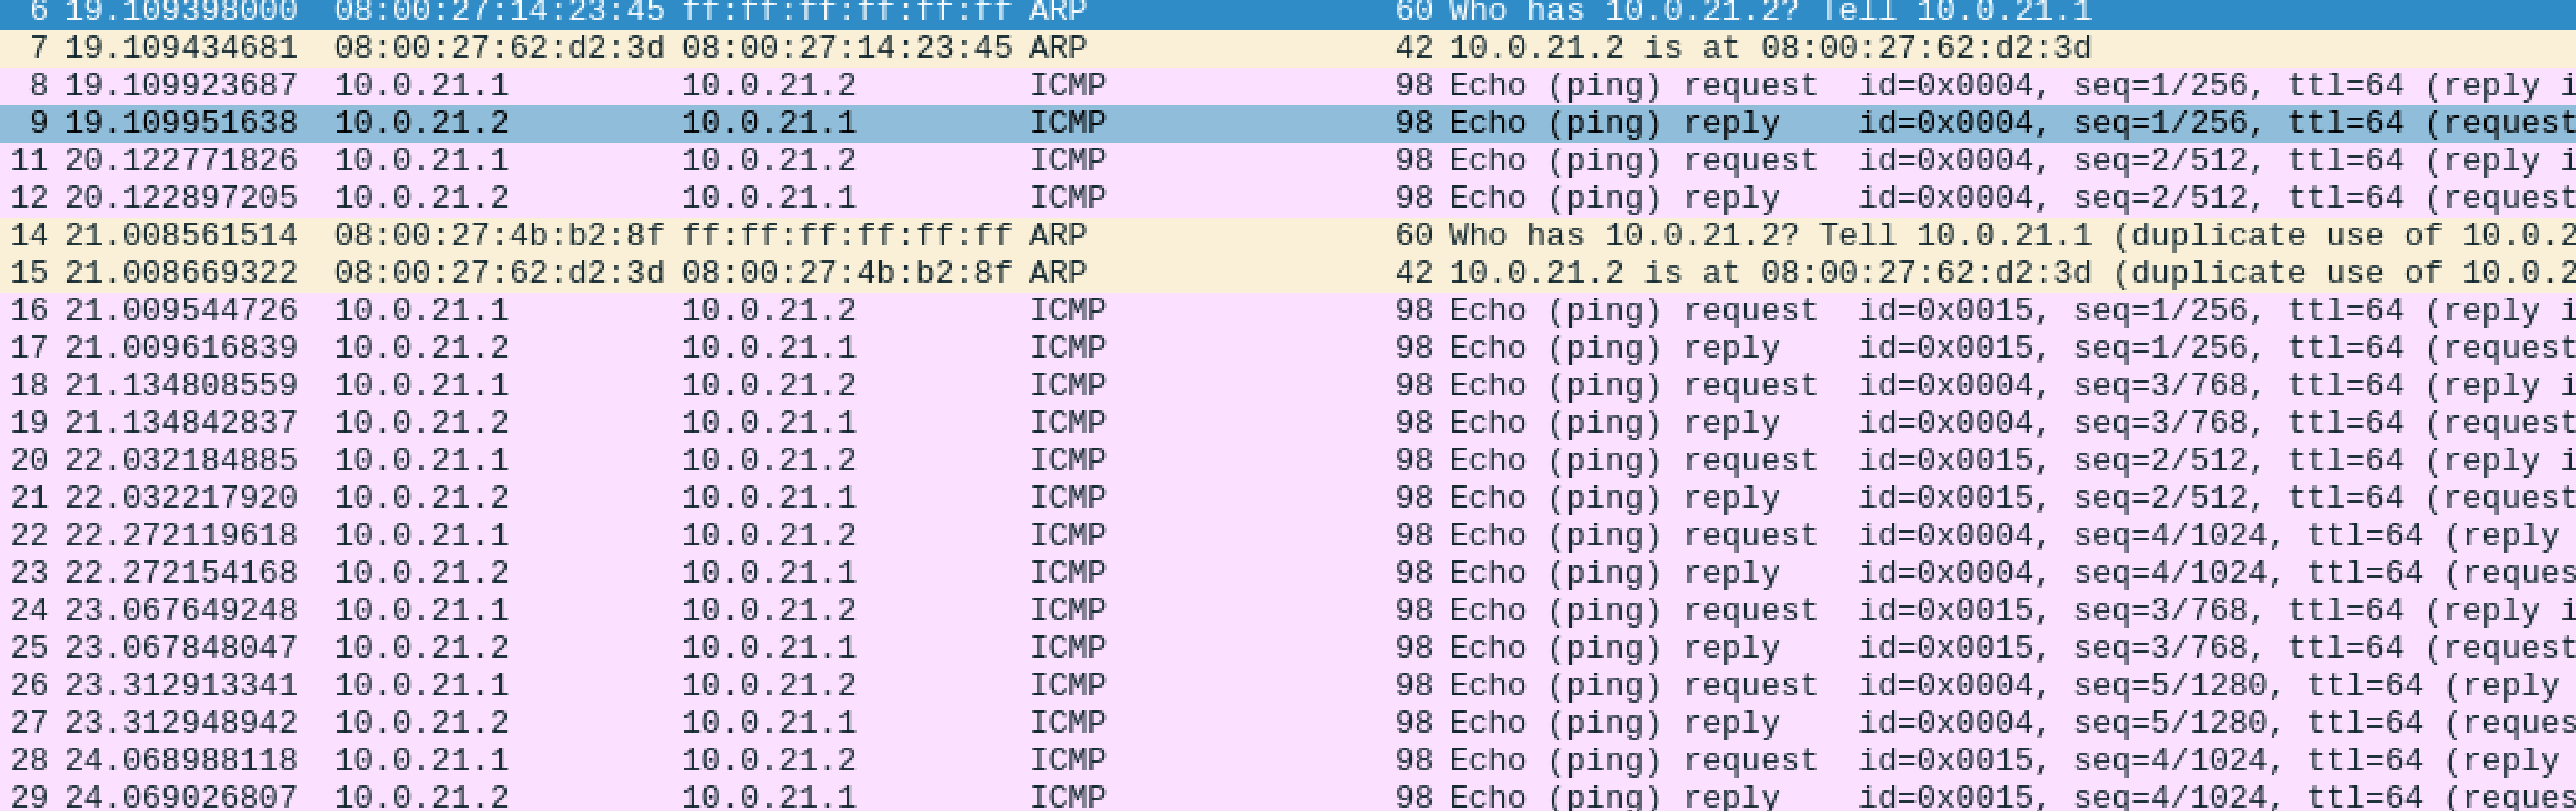
\includegraphics[width=0.75\textwidth]{es2.2host2.png}
      %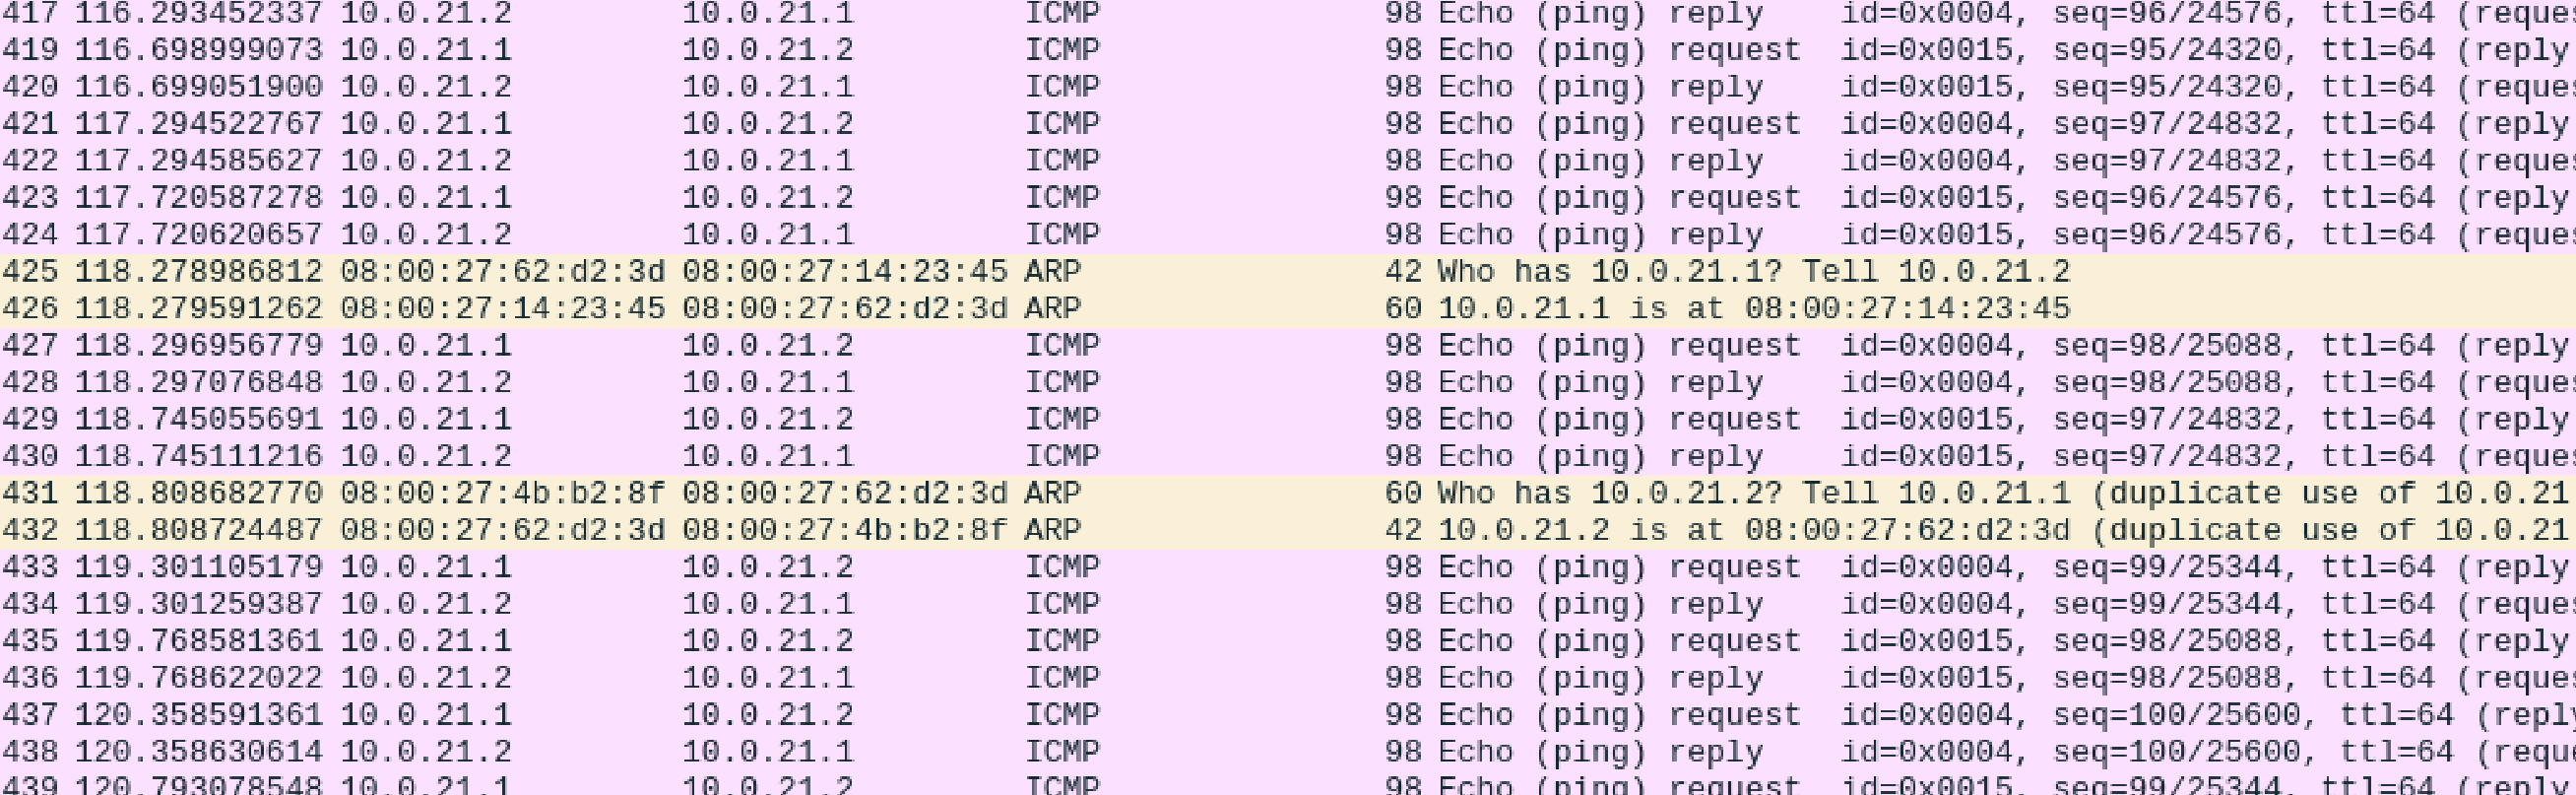
\includegraphics[width=0.75\textwidth]{Commutazione.png}
\end{wrapfigure}
Se invece eseguiamo il Ping contemporaneamente da H1 e H3 a H2, si può notare che H2 risponde in modo casuale e alternato ad entrambi.
Analizzando con wireshark il traffico in H2, notiamo all’inizio due ARP Request broadcast ad H2 a cui H2 risponda ad entrambe aggiornando conseguentemente la propria tabella alla richiesta più recente.
\pagebreak
 \begin{wrapfigure}{r}{0.75\textwidth} %this figure will be at the right
  \centering
    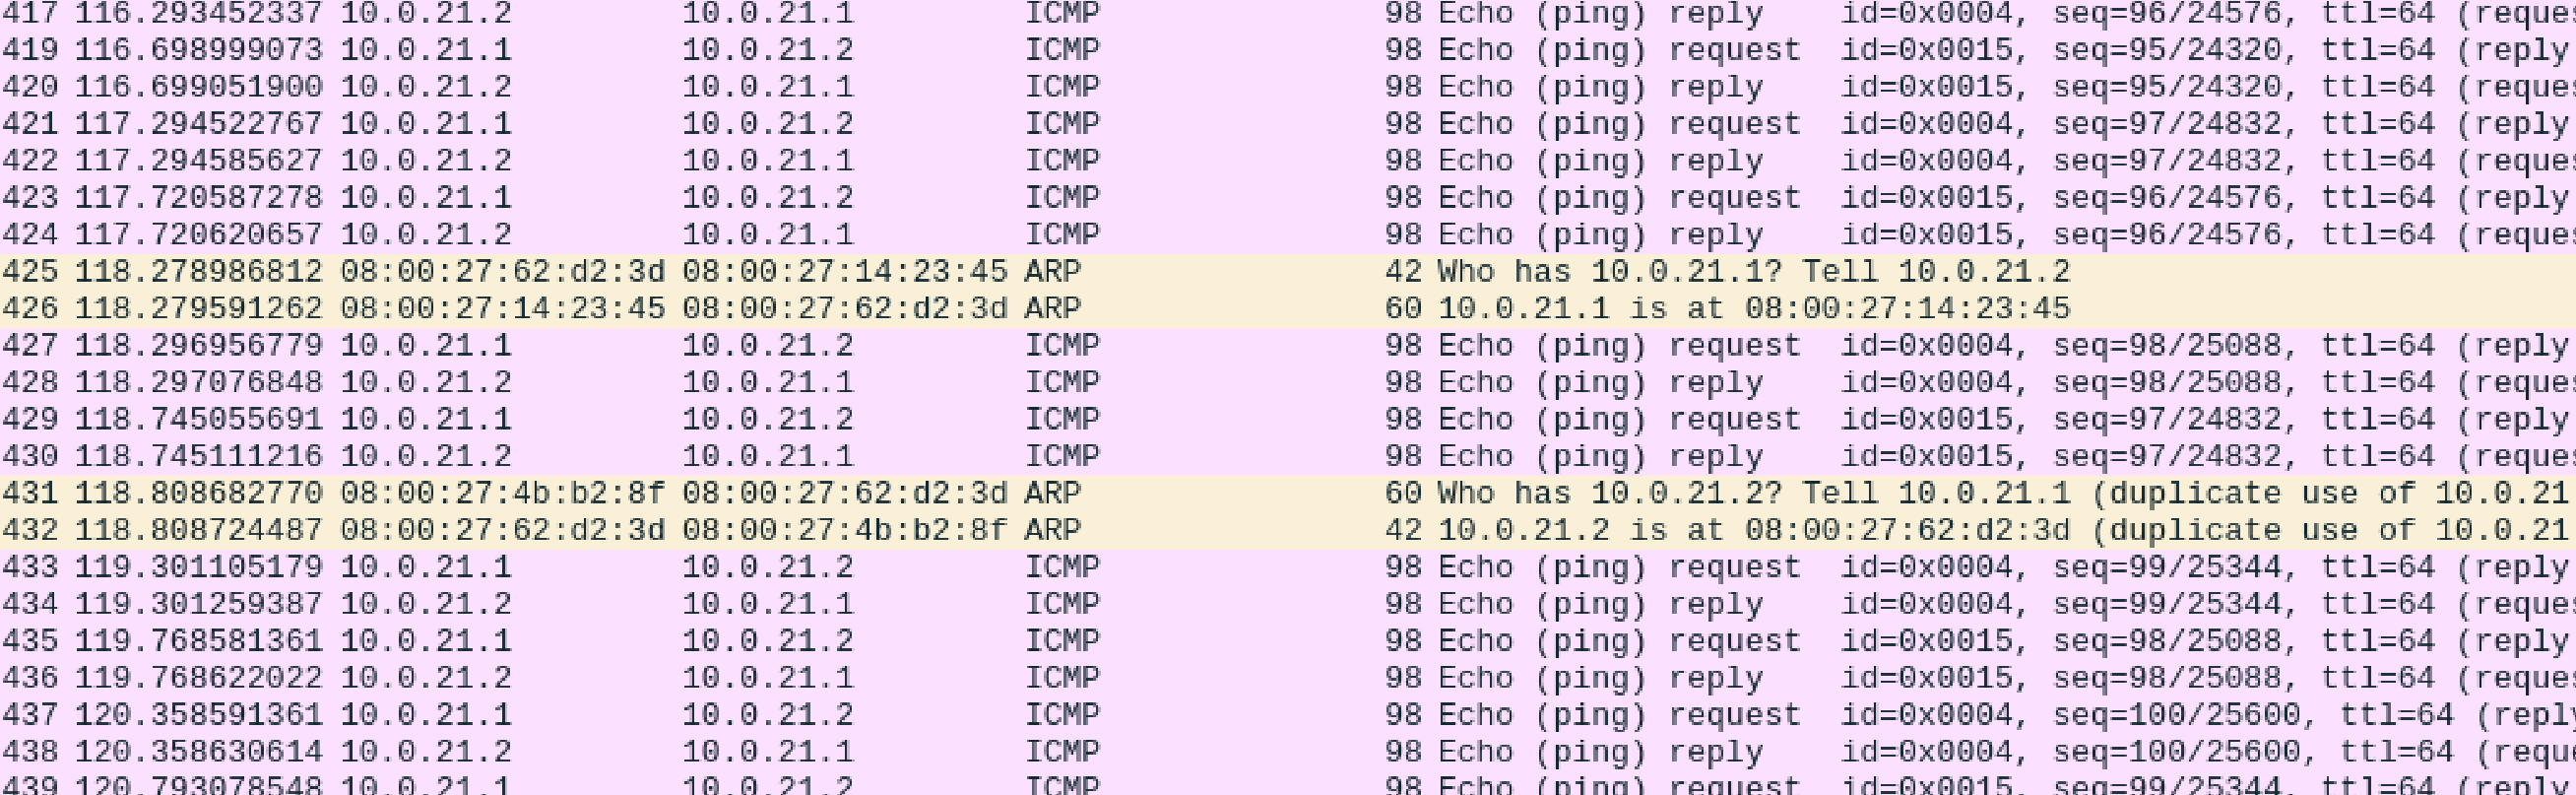
\includegraphics[width=0.75\textwidth]{Commutazione.png}
\end{wrapfigure}

H1 e H3 ad intervalli apparentemente casuali inviano con una richiesta unicast per rinfrescare la loro Arp Table ad H2 che di conseguenza aggiorna la propria tabella. Ad ogni aggiornamento, se è cambiata la tabella di ARP rispetto al momento precedente, si nota che cambiano anche le destinazioni delle Echo Reply, per questo motivo si nota l’alternanza di risposte tra H1 e H3.
I rinfreschi richiesti da H2 non modificheranno la tabella ARP, appunto perché la richiesta viene fatta in unicast.
Se analizziamo le catture sugli Host H1 e H3, si noterà che per ogni request ci saranno due reply, poiché ad H2 sono arrivate due richieste a cui rispondere. Se si riuscisse ha far partire il ping in modo contemporaneo si potrebbe apprezzare che le seconde Reply vengano definite come duplicate, ma si noterebbe anche che l’identificativo tra i due pacchetti ricevuti è diverso e solo uno corrisponde a quello dell’Host che sta effettivamente ricevendo.

Quindi le ARP table nella configurazione finale per H1 e H3 presentano l'entry che identifica H2, mentre quella di H2 conterrà il Mac dell’ultimo Host che ha fatto richiesta.

\section{Netmask sbagliate}
\begin{figure}[!htb]
    \begin{minipage}{0.48\textwidth}
        Abbiamo configurato la rete in modo che H1 veda all’interno della sua rete H2, ma H2 non veda H1 come un host appartenente alla propria sottorete.
    \end{minipage}\hfill
    \begin{minipage}{0.48\textwidth}
        \centering
        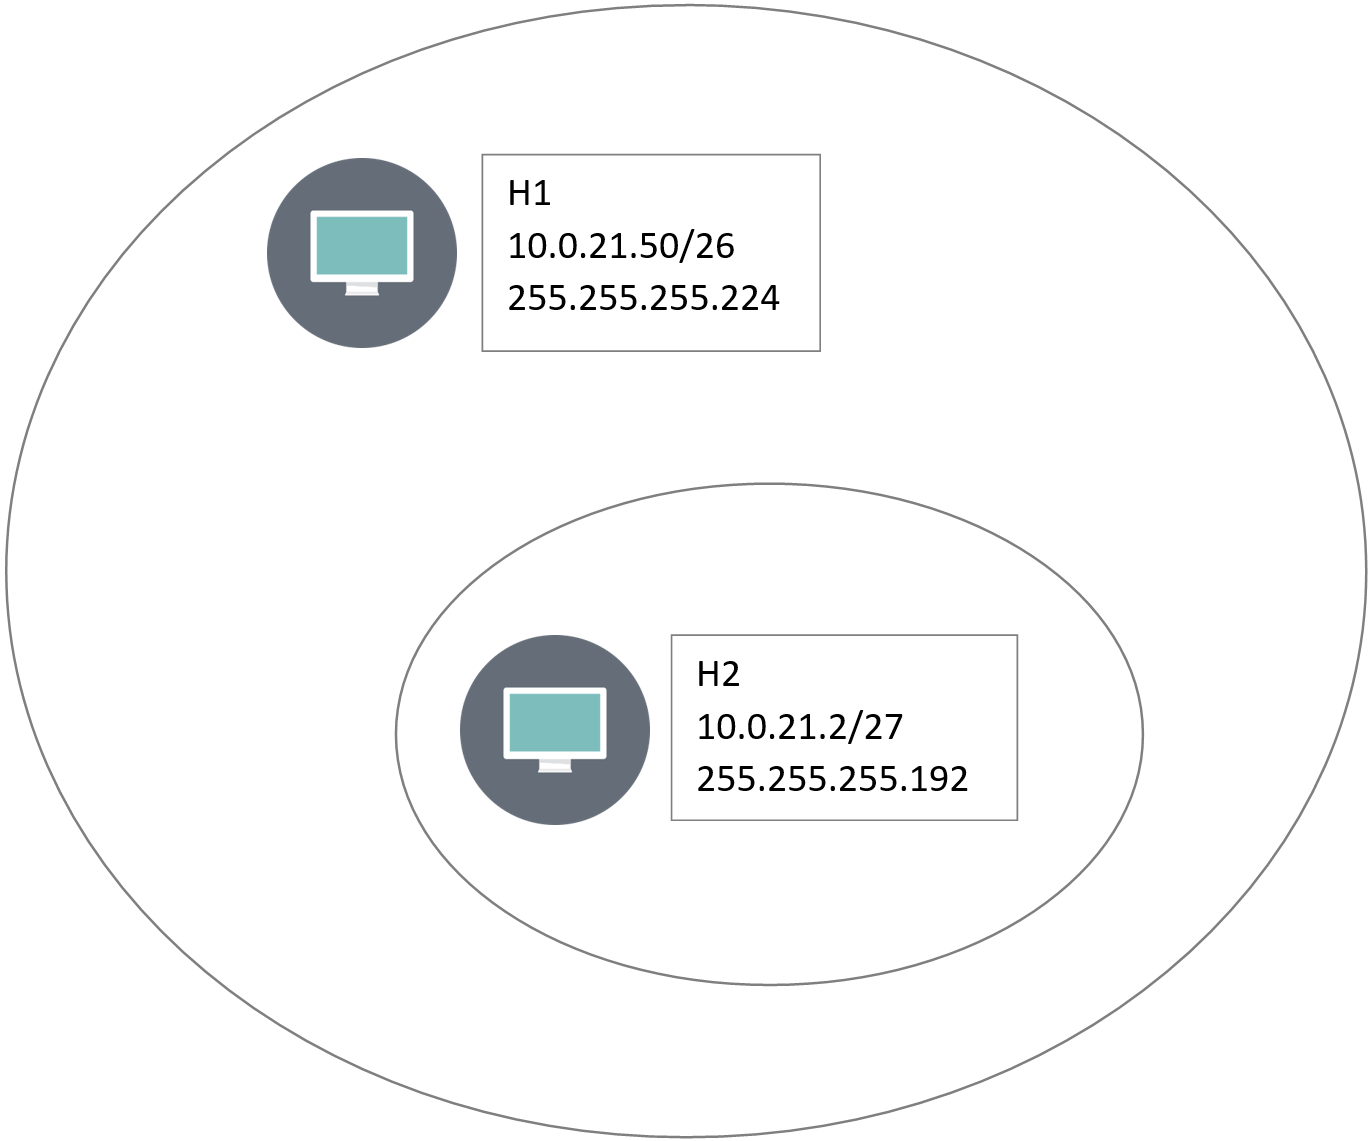
\includegraphics[width=0.7\linewidth]{es3.png}
    \end{minipage}
 \end{figure}


\subsection{Ping di H1 a H2}
\begin{figure}[!htb]
    \begin{minipage}{0.5\textwidth}
      Dal risultato si denota come H1 non riceva risposta da H2, poiché H1 manda inizialmente una ARP Request ad H2, ma H2 non potendo contattare un Host che non si trova all’interno della propria sottorete non invia nessuna \textit{ARP Reply}.
      \\La tabella ARP di H1 risulterà incompleta mentre quella di H2 risulterà vuota.
    \end{minipage}\hfill
    \begin{minipage}{0.5\textwidth}
      %\centering
      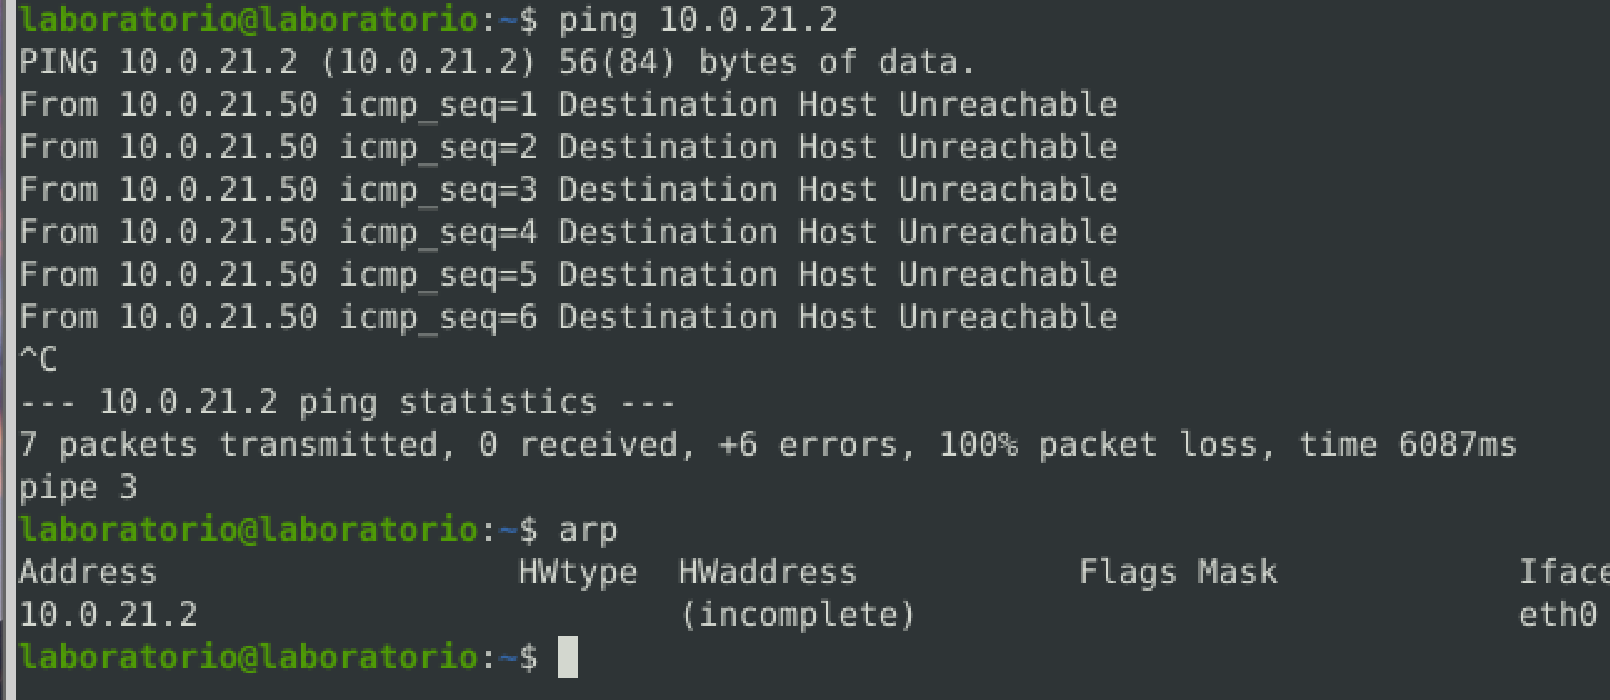
\includegraphics[width=0.8\linewidth,right]{es3hostUnreach.png}
    \end{minipage}
 \end{figure}


\subsection{Ping di H2 a H1}
\begin{figure}[!htb]
    \begin{minipage}{0.55\textwidth}
      H2 non può inviare nessuna ARP Request verso H1, e non essendo impostato nessun default gateway non può raggiungere nessun host esterno alla rete.
      Entrambe le ARP Table risulteranno quindi vuote.
    \end{minipage}\hfill
    \begin{minipage}{0.4\textwidth}
      \centering
      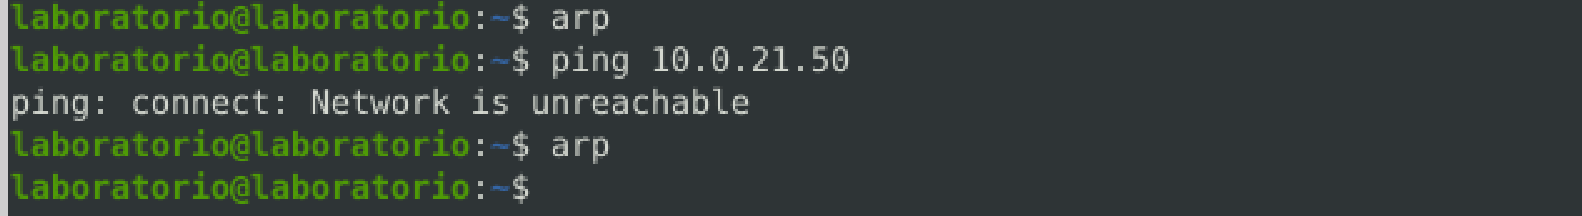
\includegraphics[width=1\linewidth]{es3NetworkUnreach.png}
    \end{minipage}
 \end{figure}
 \pagebreak
\section{Netmask sbagliate e broadcast in conflitto}
\begin{figure}[!htb]
    \begin{minipage}{0.48\textwidth}
    Abbiamo configurato la rete in modo che H1 veda all’interno della propria rete H2, ma H1 è l’indirizzo broadcast della sottorete di H2.
    \end{minipage}\hfill
    \begin{minipage}{0.48\textwidth}
      \centering
      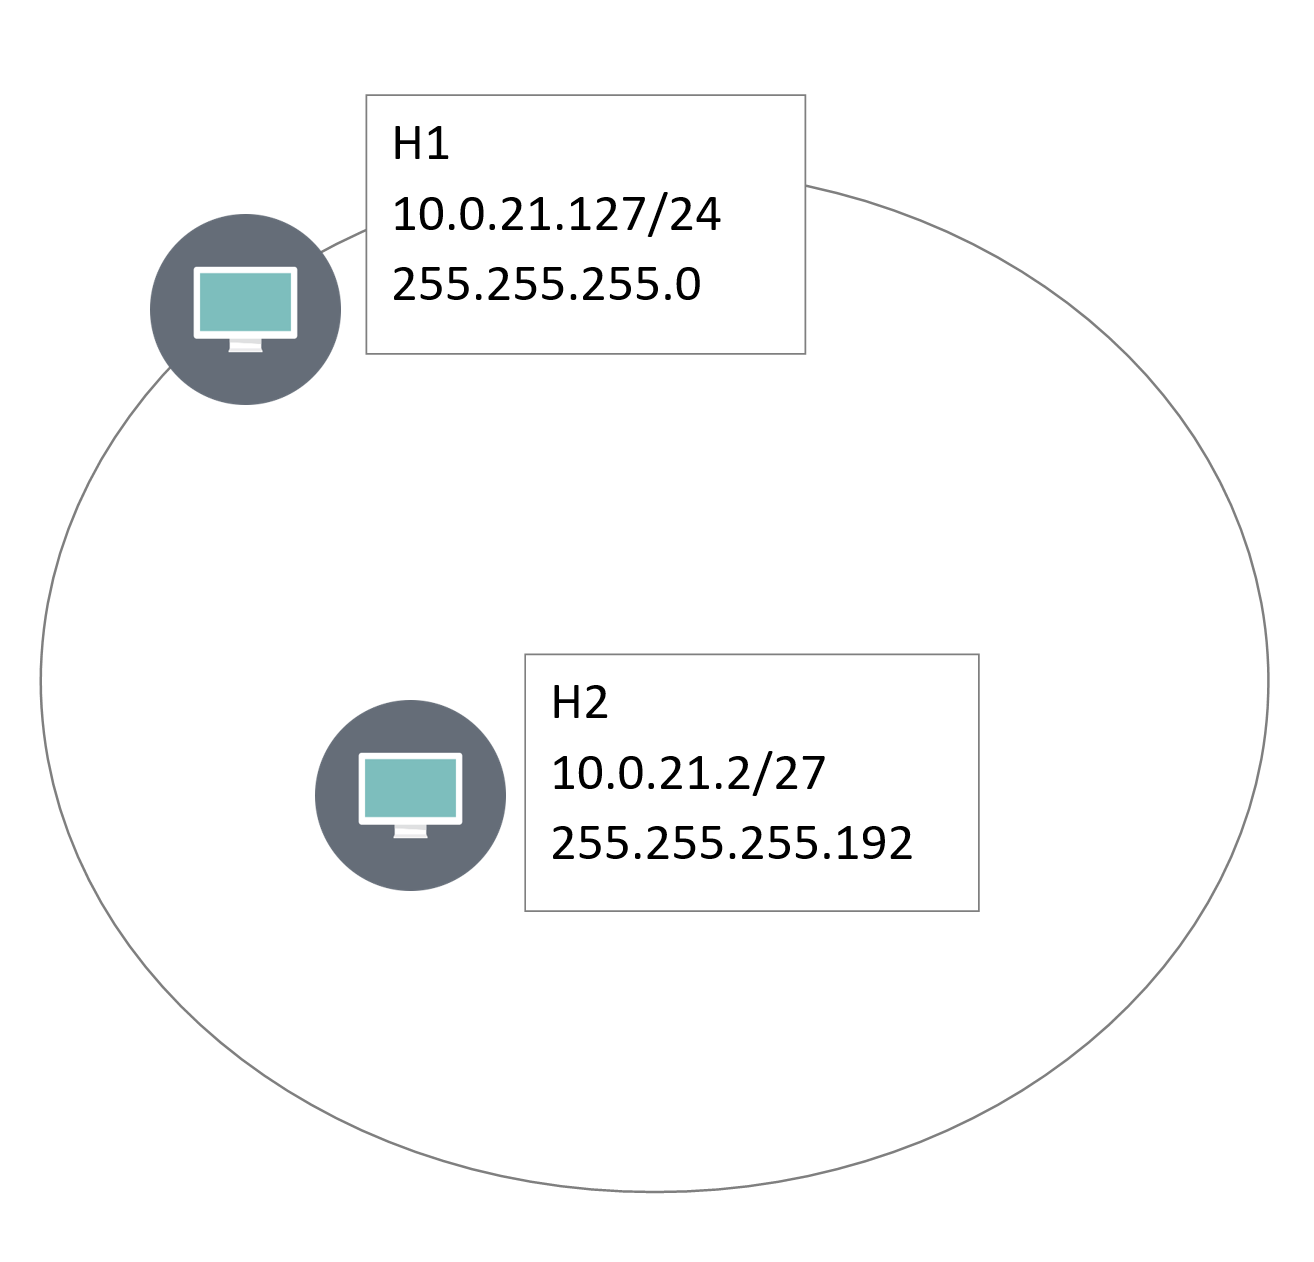
\includegraphics[width=0.7\linewidth]{es4.png}
    \end{minipage}
 \end{figure}

 \subsection{Ping di H1 a H2}

 \begin{figure}[!htb]
    \begin{minipage}{0.2\textwidth}
        In questo caso si è violata la semantica per la \textit{ARP Request} poiché l’indirizzo di \textit{Source} è quello di broadcast della sottorete di H2,quindi H2 non può rispondere alla richiesta.
        Le tabelle di ARP H1 sarà incompleta e quella di H2 sarà vuota.  
    \end{minipage}\hfill
    \begin{minipage}{0.78\textwidth}
      \centering
      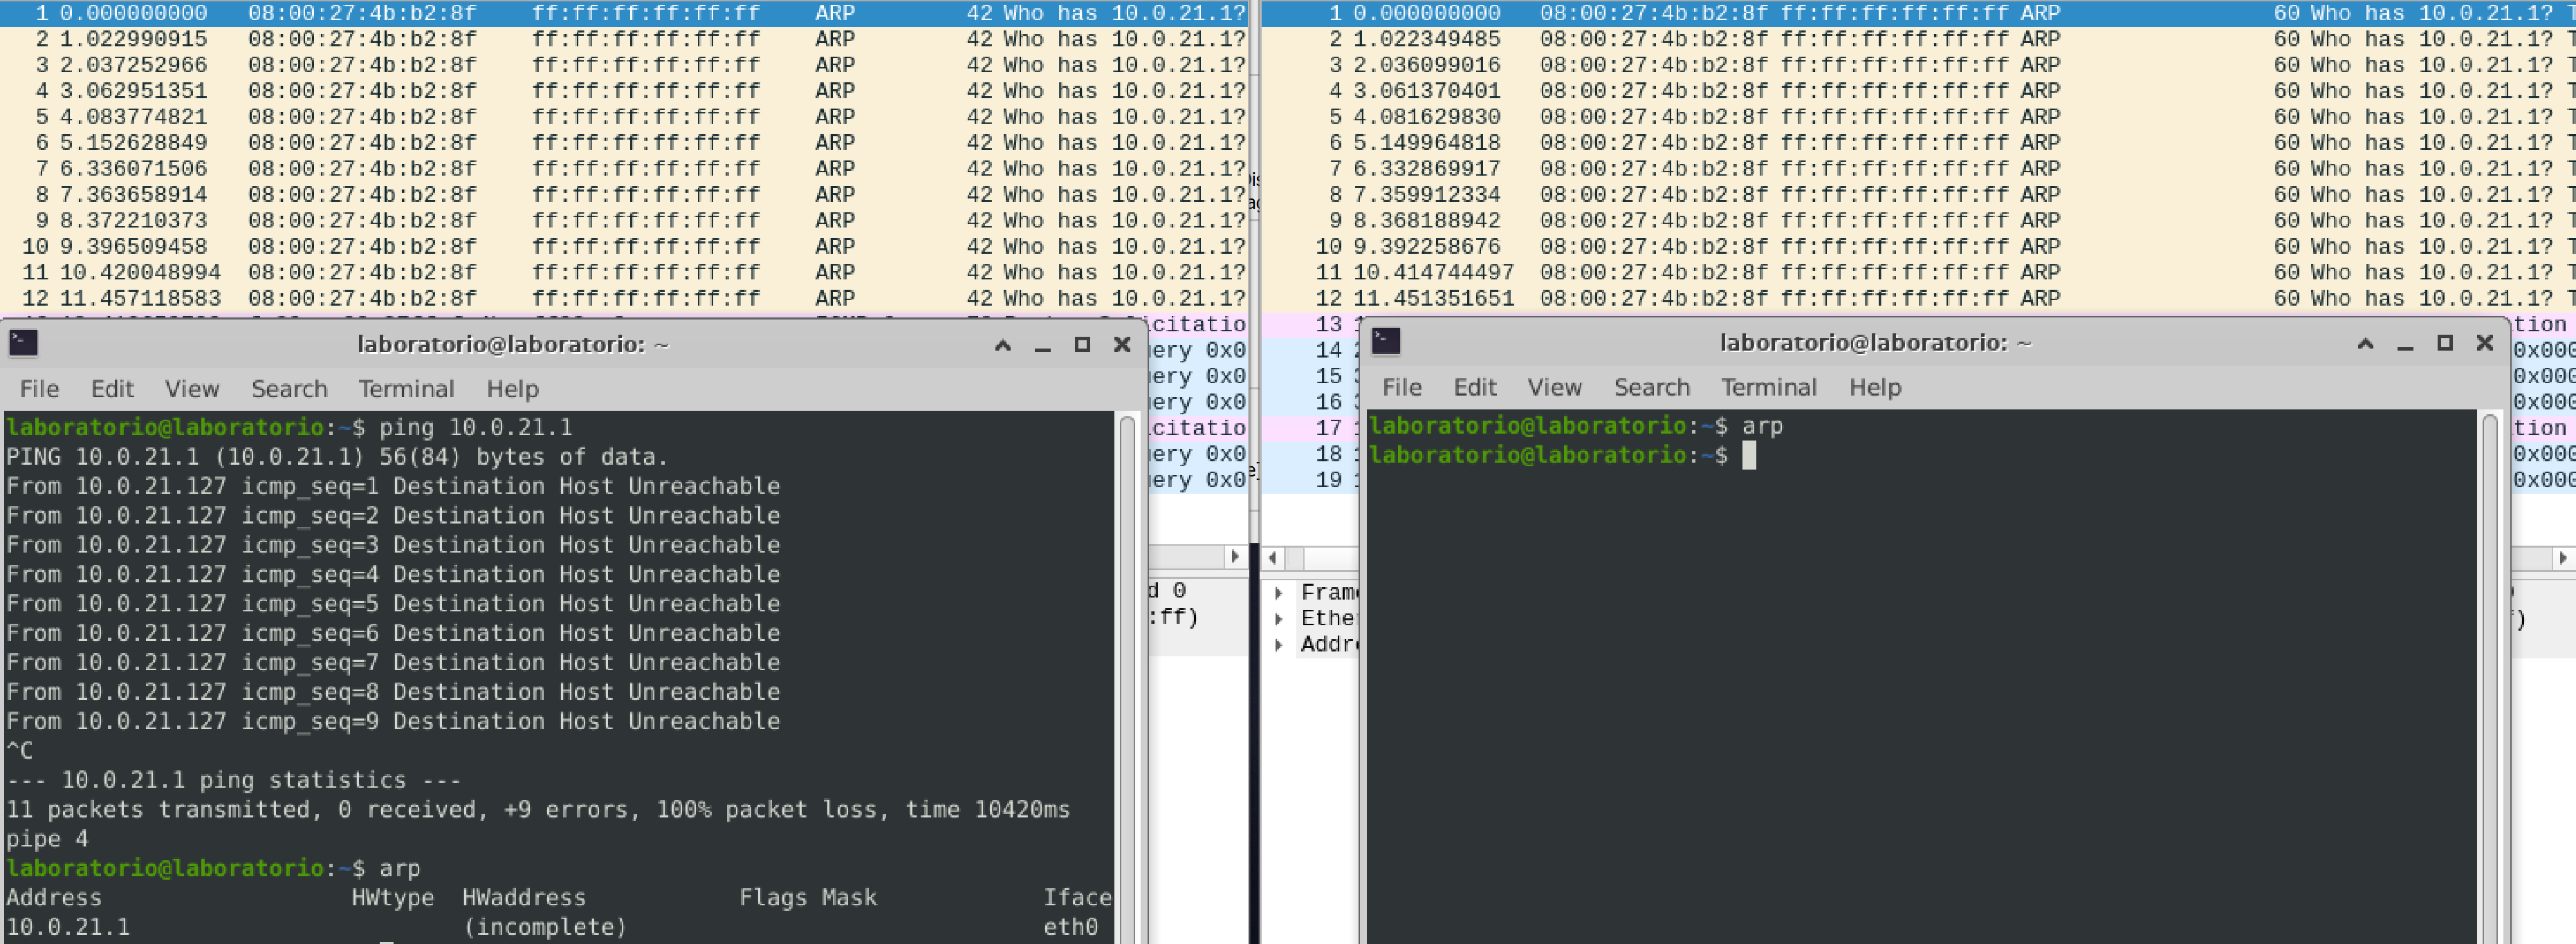
\includegraphics[width=1.05\linewidth]{es4.1.png}
    \end{minipage}
 \end{figure}

 \subsection{Ping di H2 a H1}

 Per effettuare questo ping bisogna utilizzare l’opzione -b per abilitare il ping al broadcast.
Le uniche risposte che riceverà sono quelle relative all’interfaccia di loopback, mentre non riceverà risposte da H1 perché per lo stesso motivo del punto precedente si sta violando la semantica della \textit{ARP Request}: H1 è sempre l’indirizzo di broadcast della sottorete di H2.
Le ARP Table quindi risultano uguali al punto precedente perché H2 non risponderà alla ARP Request di H1.


 \begin{figure}[!htb]
    \begin{minipage}{0.49\textwidth}
      \centering
      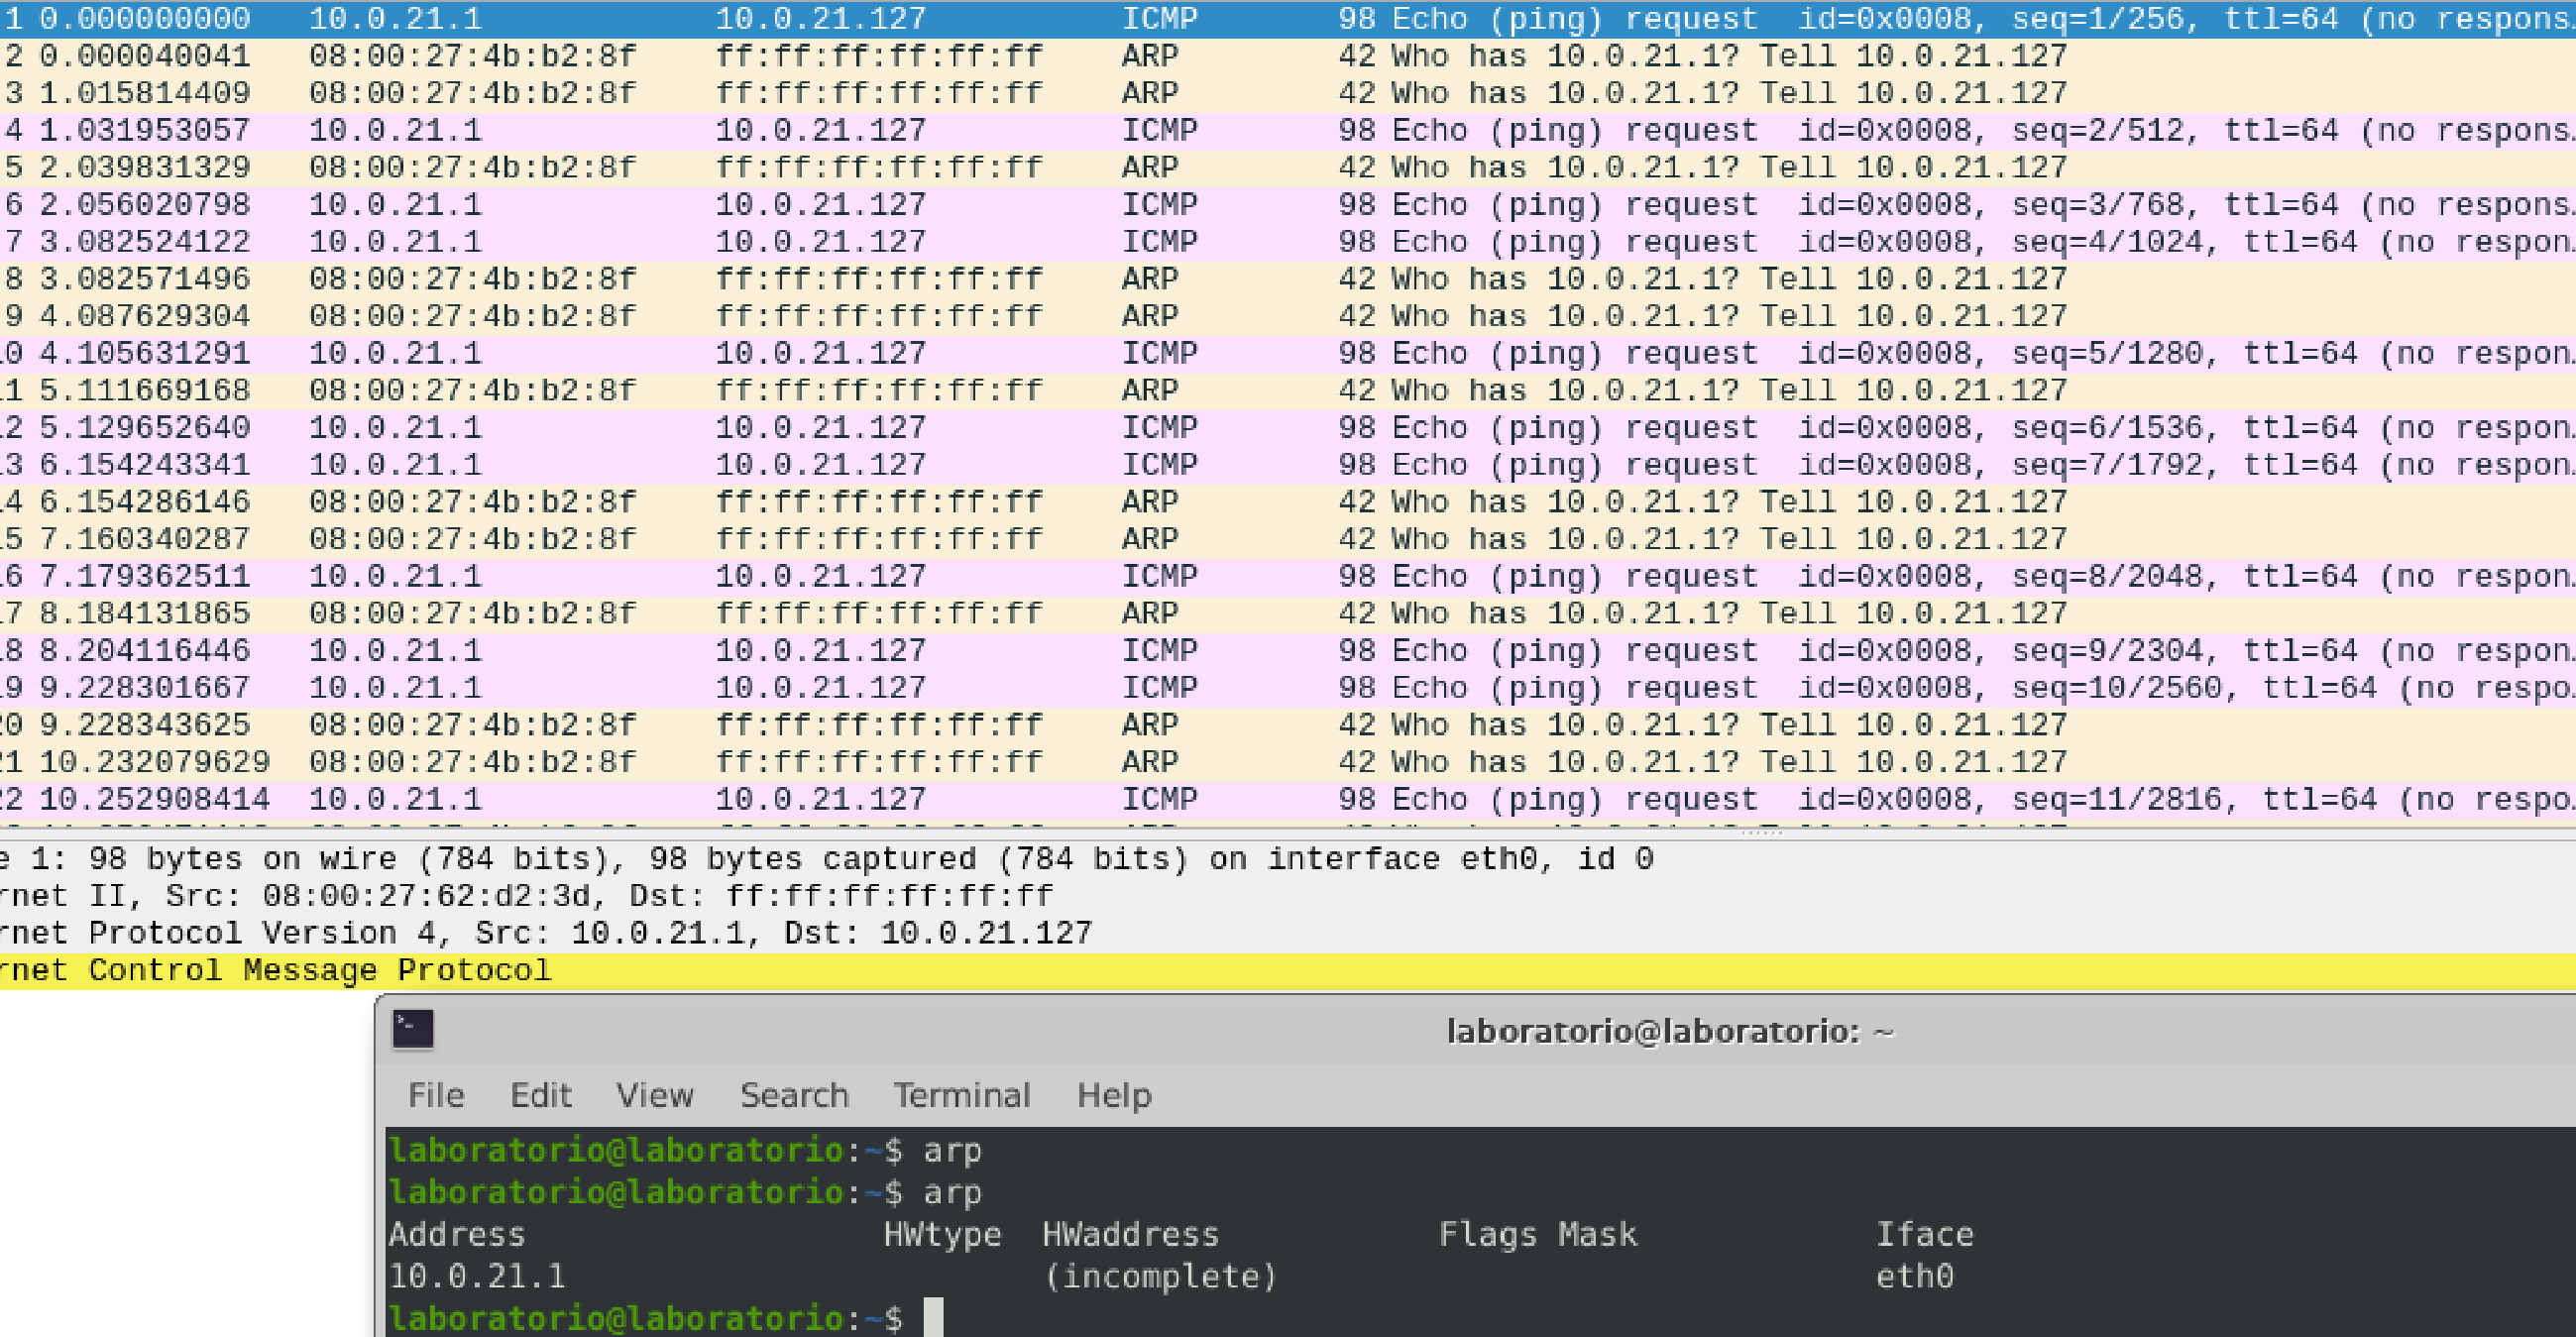
\includegraphics[width=1\linewidth]{es4.2.1.png}
    \end{minipage}\hfill
    \begin{minipage}{0.49\textwidth}
      \centering
      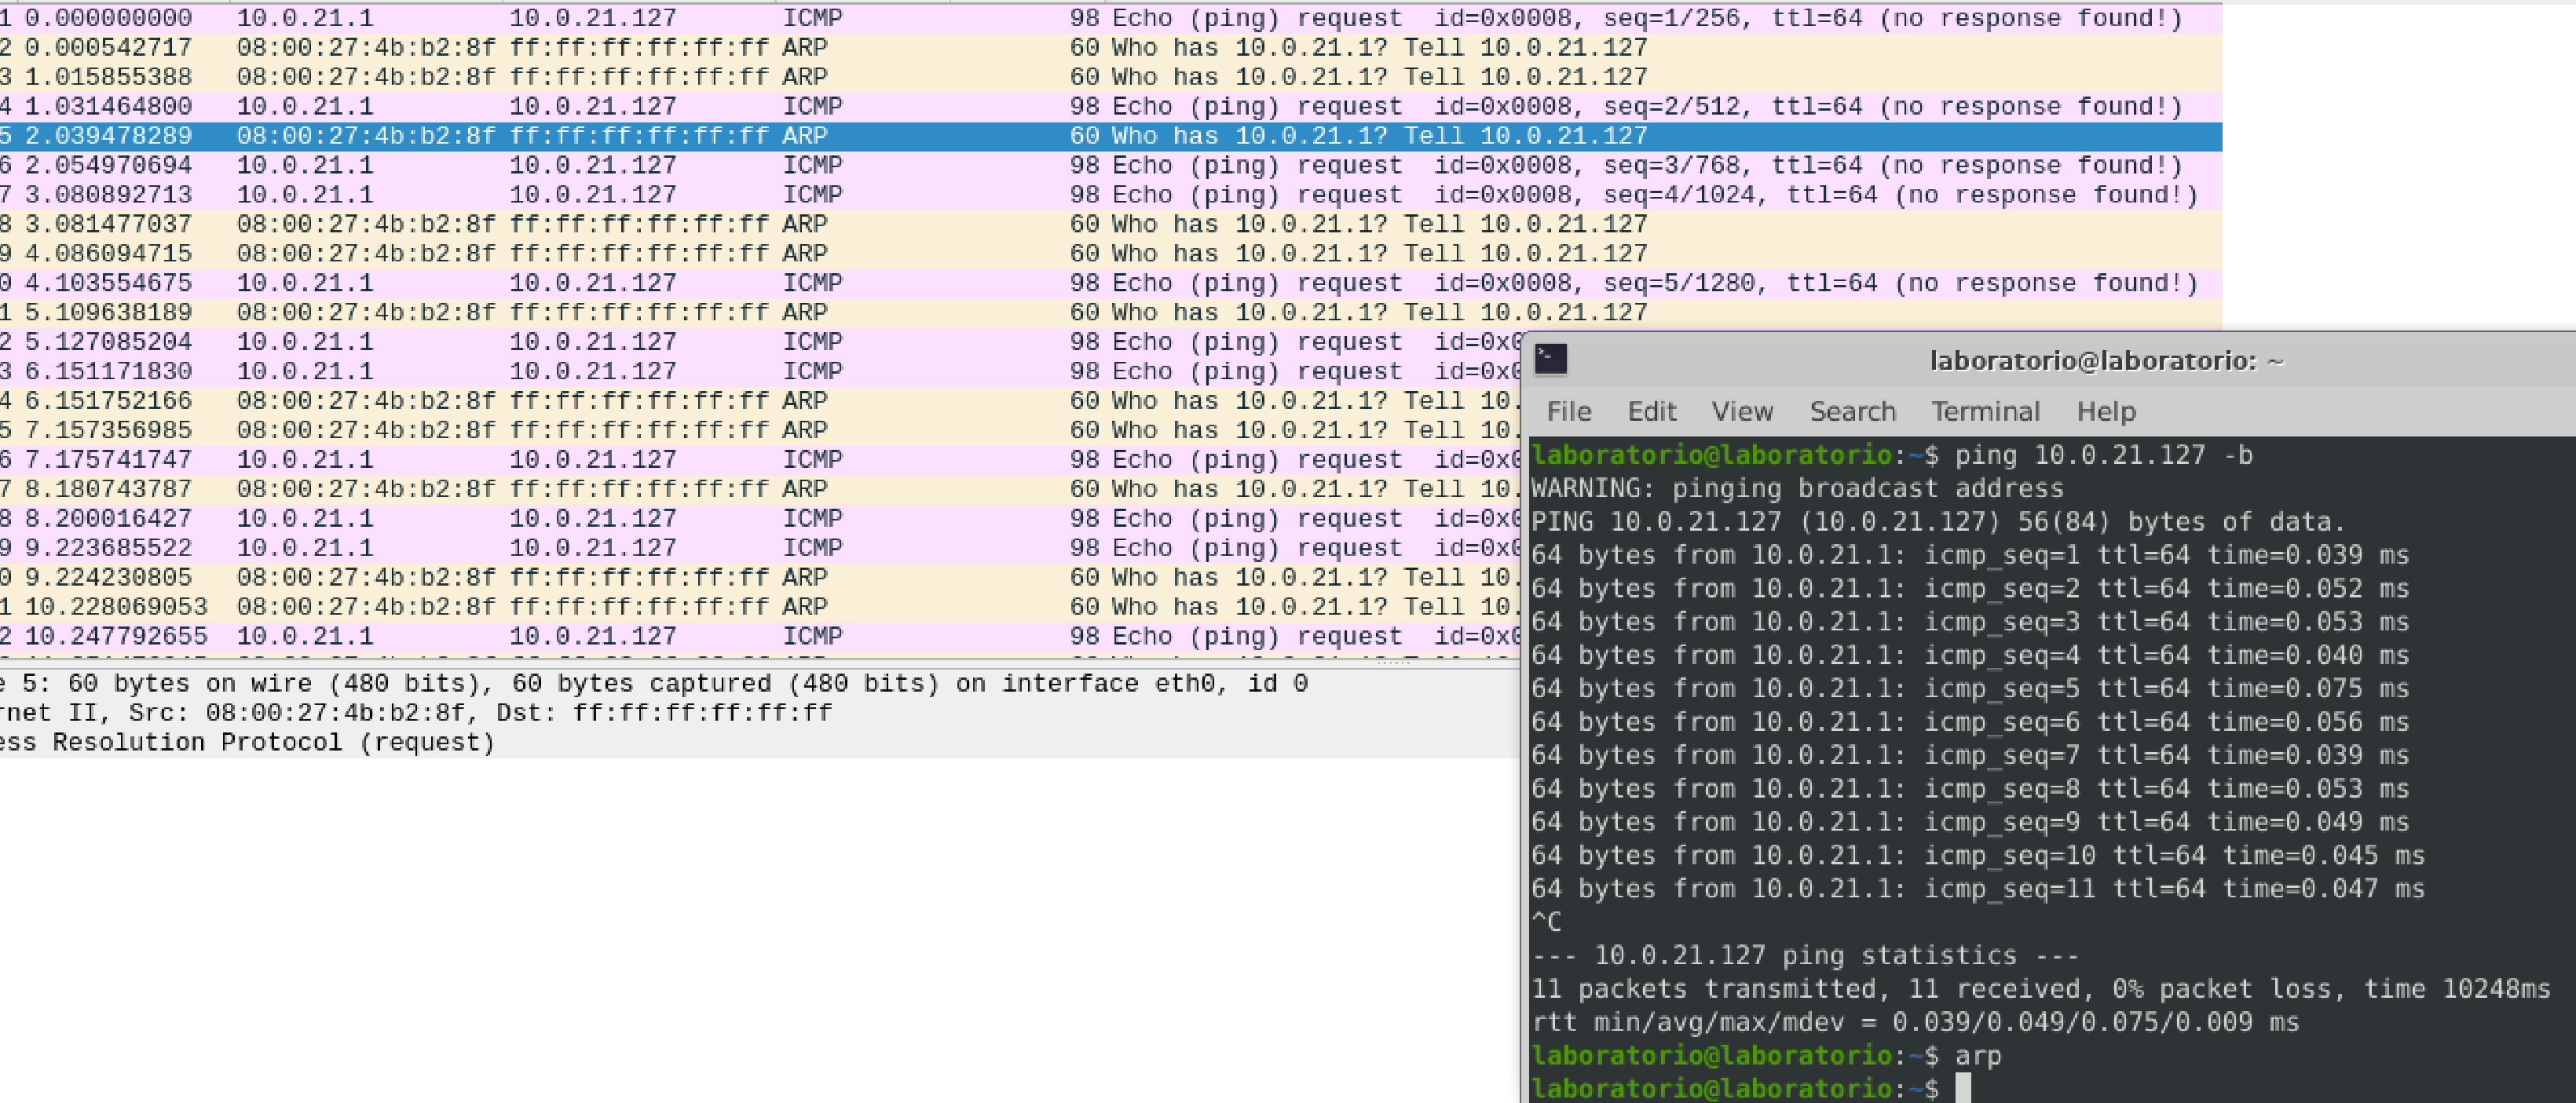
\includegraphics[width=1\linewidth]{es4.2.2.png}
    \end{minipage}
 \end{figure}
\end{document}